\ifx\allfiles\undefined
\documentclass[11 pt,t]{beamer}
\geometry{showframe,paperwidth=160mm,paperheight=120mm,margin=5mm,nohead,nofoot,nomarginpar}
%\usetheme[
%bullet=circle,		% Other option: square
%bigpagenumber,		% circled page number on lower right
%topline=true,		% colored bar at the top of the frame 
%]{Zurich}

\usetheme{metropolis}

\usepackage{amsmath}
\usepackage{fontspec,xunicode,xltxtra}
\usepackage{pgf}
\usepackage{tikz}
\usetikzlibrary{patterns}
\usetikzlibrary{plotmarks}
\usetikzlibrary{arrows,decorations.pathmorphing,backgrounds,fit,positioning,shapes,chains}
\definecolor{yellow1}{rgb}{1,0.8,0.2}  
\usepackage{pgfplots}
\pgfplotsset{compat=newest}
\tikzset{elegant/.style={smooth,thick,samples=50,cyan}}
\tikzset{eaxis/.style={->,>=stealth}}

\let\oldequation=\equation
\let\oldendequation=\endequation
\renewenvironment{equation}{\oldequation\textstyle}{\oldendequation}
\setlength{\baselineskip}{0pt}
\renewcommand{\baselinestretch}{0pt}
\setlength{\partopsep}{0pt}
\setlength{\parsep}{0pt}
\setlength{\itemsep}{0cm}
\setlength{\topsep}{0cm}
\setlength{\parskip}{0pt}
\setlength{\lineskip}{0pt}
%\setitemize[1]{itemsep=0pt,partopsep=0pt,parsep=\parskip,topsep=0pt}
%%\usepackage[compatibility=false]{caption}
%%\captionsetup{font={scriptsize}}
\setbeamerfont{caption}{size=\tiny}
\setlength{\abovecaptionskip}{0pt}
\setlength{\belowcaptionskip}{0pt}
\setlength{\abovedisplayshortskip}{0pt}
\setlength{\belowdisplayshortskip}{0pt}
\setlength{\abovedisplayskip}{0pt}
\setlength{\belowdisplayskip}{0pt}
\setlength{\jot}{0pt}
\usepackage{setspace} 
\linespread{1.4}
\fi

\def\allfiles{allfiles}
%-----------------------------------------------------------------------------
% DOCUMENT PROPERTIES

\author{Huang Yuefeng}
\title{Introduction to Machine Learning}

%-----------------------------------------------------------------------------

\begin{document}

% ----------------------------------------------------------------------------
\frame{

	\titlepage
}
% ----------------------------------------------------------------------------
\setcounter{tocdepth}{1}
\frame[shrink]
{
\frametitle{Guideline}
\tableofcontents
}
% ----------------------------------------------------------------------------
\ifx\allfiles\undefined
\documentclass[11 pt,t]{beamer}
\geometry{showframe,paperwidth=160mm,paperheight=120mm,margin=5mm,nohead,nofoot,nomarginpar}
%\usetheme[
%bullet=circle,		% Other option: square
%bigpagenumber,		% circled page number on lower right
%topline=true,		% colored bar at the top of the frame 
%]{Zurich}

\usetheme{metropolis}

\usepackage{amsmath}
\usepackage{fontspec,xunicode,xltxtra}
\usepackage{pgf}
\usepackage{tikz}
\usetikzlibrary{patterns}
\usetikzlibrary{plotmarks}
\usetikzlibrary{arrows,decorations.pathmorphing,backgrounds,fit,positioning,shapes,chains}
\definecolor{yellow1}{rgb}{1,0.8,0.2}  
\usepackage{pgfplots}
\pgfplotsset{compat=newest}
\tikzset{elegant/.style={smooth,thick,samples=50,cyan}}
\tikzset{eaxis/.style={->,>=stealth}}

\let\oldequation=\equation
\let\oldendequation=\endequation
\renewenvironment{equation}{\oldequation\textstyle}{\oldendequation}
\setlength{\baselineskip}{0pt}
\renewcommand{\baselinestretch}{0pt}
\setlength{\partopsep}{0pt}
\setlength{\parsep}{0pt}
\setlength{\itemsep}{0cm}
\setlength{\topsep}{0cm}
\setlength{\parskip}{0pt}
\setlength{\lineskip}{0pt}
%\setitemize[1]{itemsep=0pt,partopsep=0pt,parsep=\parskip,topsep=0pt}
%%\usepackage[compatibility=false]{caption}
%%\captionsetup{font={scriptsize}}
\setbeamerfont{caption}{size=\tiny}
\setlength{\abovecaptionskip}{0pt}
\setlength{\belowcaptionskip}{0pt}
\setlength{\abovedisplayshortskip}{0pt}
\setlength{\belowdisplayshortskip}{0pt}
\setlength{\abovedisplayskip}{0pt}
\setlength{\belowdisplayskip}{0pt}
\setlength{\jot}{0pt}
\usepackage{setspace} 
\linespread{1.4}
\fi

\ifx\allfiles\undefined
\begin{document}
\fi
\section{Introduction}
% ----------------------------------------------------------------------------
\begin{frame}
\frametitle{Introduction of Machine Learning}
\framesubtitle{Problem Definition}
	\small
	\begin{itemize}
		\item hypothesis function: $h_{\theta}:X \rightarrow Y$
		\item loss function: $L:Y,h_{\theta}(X) \rightarrow R$, where $R$ is real number.
		\item log loss function: $l:log(L)$ 
		\item training set: a list of $m$ training example $\{x^{(i)},y^{(i)}\}$, $y^{(i)}$ called label of $x^{(i)}$
		\item machine learning = training + predicting
		\item training: try to get $\theta$ at minimum value of $L$ by using $\{x^{(i)},y^{(i)}\}$ and Convex Optimization method
		\item predicting: use $h$ with $\theta$ to predict $y$ of unknown $x$
	\end{itemize}
\end{frame}
% ----------------------------------------------------------------------------
% ----------------------------------------------------------------------------

\begin{frame}
\centering
\frametitle{Core Knowledge}
\begin{tikzpicture}
[auto,
decision/.style={diamond, draw=blue, thick, fill=blue!20,
text width=4.5em,align=flush center,
inner sep=1pt},
block/.style ={circle, fill=yellow1,
text width=5em,align=center, rounded corners,
minimum size=1cm, inner sep=1, text width=1cm},
line/.style ={draw, thick, -latex’,shorten >=2pt},
cloud/.style ={draw=black!20, ellipse,fill=green!20,
minimum height=2cm}, minimum width=6cm]
%[->,>=stealth',shorten >=1pt,auto,node distance=2.8cm,semithick]  
%\tikzstyle{every node}=[circle,fill=yellow1,text=black,align=center,minimum size=1cm,inner sep=1,text width=1cm]   
\tiny
%\filldraw[draw=black!20, fill=green!20, minimum size=3cm] (8,-1) ellipse (2.5 and 1);
\node [cloud](c) at (8,-1) {};
\node [block]                (la)    at (6.5, -1)             {linear\\algebra};  
\node [block]                (pt)    at (8, -1)             {probability\\theory};  
\node [block]                (co)    at (9.5, -1)             {convex\\optimization};  
\node [block]                (lir)    at (4.5, -3)             {linear\\regression};  
\node [block]                (lr)    at (4.5, -4.5)             {logistic\\regression};  
\node [block]                (svm)   at (4.5, -7.5)             {SVM};
\node [block]                (sr)    at (4.5, -6)             {softmax\\regression};  

\node [block]                (nb)    at (8, -3)             {naive\\bayes};  
\node [block]                 (em)    at (8, -4.5)             {EM};  
\node [block]                (me)   at (8, -6)             {maximum\\entropy};
\node [block]                (hmm)    at (8, -7.5)             {HMM};  

\node [block]                (nn)    at (11.5, -3)             {neutral\\network};  
\node [block]                (dnn)    at (11.5, -4.5)             {DNN};  
\node [block]                (cnn)    at (11.5, -6)             {CNN};  
\node [block]                (rnn)    at (11.5, -7.5)             {RNN};  

\draw  [->] (c) to (lir);
\draw  [->] (lir) to (lr);
\draw  [->] (lr) to (sr);
\draw  [->] (sr) to (svm);


\draw  [->] (c) to (nb);
\draw  [->] (nb) to (em);
\draw  [->] (em) to (me);
\draw  [->] (me) to (hmm);

\draw  [->] (c) to (nn);
\draw  [->] (nn) to (dnn);
\draw  [->] (dnn) to (cnn);
\draw  [->] (cnn) to (rnn);

\end{tikzpicture} 
\end{frame}
% ----------------------------------------------------------------------------
\ifx\allfiles\undefined
\end{document}
\fi

%\ifx\allfiles\undefined
\documentclass[11 pt,t]{beamer}
\usetheme[
%bullet=circle,		% Other option: square
%bigpagenumber,		% circled page number on lower right
%topline=true,		% colored bar at the top of the frame 
%]{Zurich}

\usetheme{metropolis}

\usepackage{amsmath}
\usepackage{fontspec,xunicode,xltxtra}
\usepackage{pgf}
\usepackage{tikz}
\usetikzlibrary{patterns}
\usetikzlibrary{plotmarks}
\usetikzlibrary{arrows,decorations.pathmorphing,backgrounds,fit,positioning,shapes,chains}
\definecolor{yellow1}{rgb}{1,0.8,0.2}  %opening 
\usepackage{pgfplots}
\pgfplotsset{compat=newest}
\tikzset{elegant/.style={smooth,thick,samples=50,cyan}}
\tikzset{eaxis/.style={->,>=stealth}}


\let\oldequation=\equation
\let\oldendequation=\endequation
\renewenvironment{equation}{\oldequation\textstyle}{\oldendequation}
\setitemize[1]{itemsep=5pt,partopsep=0pt,parsep=\parskip,topsep=3pt}
%\usepackage[compatibility=false]{caption}
%\captionsetup{font={scriptsize}}
\setbeamerfont{caption}{size=\tiny}
\setlength{\abovecaptionskip}{0pt}
\setlength{\belowcaptionskip}{0pt}
\setlength{\abovedisplayshortskip}{0pt}
\setlength{\belowdisplayshortskip}{0pt}
\setlength{\abovedisplayskip}{0pt}
\setlength{\belowdisplayskip}{0pt}
\setlength{\jot}{0pt}
\begin{document}
\fi
% ----------------------------------------------------------------------------
\begin{frame}
\frametitle{Linear Regression}
	\small 
	\begin{itemize}
		\item Problem Definition\\
			\footnotesize
			Draw a line to fix the distribution of dots as much as possible.\\
			If coordinates of dots are given, how to determine the optimal line?
	\end{itemize}
	\centering 
	\begin{tikzpicture}
		\begin{axis}[xlabel={$x_1$},ylabel={$x_2$},
					]
		\addplot[domain=0:10]
			{3*x+1};
		\addplot[draw=green]
%horizontal lines, vertical lines, north east lines, north west lines, grid, crosshatch, dots, crosshatch dots, fivepointed stars, sixpointed stars, bricks, checkerboard
			coordinates
			{
				(0,0)
			};
		\end{axis}
	\end{tikzpicture}
\end{frame}
\begin{frame}
			  \begin{tikzpicture}[->,>=stealth',shorten >=1pt,auto,node distance=2.8cm,semithick]  
			  \begin{axis}
			  [
			  title={f1 by threshold},
			  xlabel={Threshold},
			  ylabel={F1},
			  xmin=0, xmax=1,
			  ymin=0, ymax=1,
			  xtick={0,0.1,0.2,0.3,0.4,0.5,0.6,0.7,0.8,0.9,1},
			  ytick={0,0.1,0.2,0.3,0.4,0.5,0.6,0.7,0.8,0.9,1},
			  legend pos=north west,
			  ymajorgrids=true,
			  grid style=dashed,
			  width=15cm, height=10cm, tick align=outside, xstep=0.05,ystep=0.05
			  ]
\centering
			  \addplot[green, mark=triangle*] 
			  coordinates 
{
	(0.0,0.98066298342541436463)
		(0.05,0.98066298342541436463)
		(0.10,0.98066298342541436463)
		(0.15,0.98066298342541436463)
		(0.20,0.98066298342541436463)
		(0.25,0.98066298342541436463)
		(0.30,0.97925311203319502073)
		(0.35,0.97783933518005540164)
		(0.40,0.97571131158917418458)
		(0.45,0.97499999999999999999)
		(0.50,0.96710986703988803358)
		(0.55,0.96202531645569620252)
		(0.60,0.94571428571428571427)
		(0.65,0.92262773722627737225)
		(0.70,0.88097043214556482183)
		(0.75,0.83596214511041009463)
		(0.80,0.75359864521591871294)
		(0.85,0.73212747631352282513)
		(0.90,0.70877192982456140350)
		(0.95,0.38316722037652270209)
		(01.00,0.0)
};
\end{axis}
\end{tikzpicture} 
%\begin{tikzpicture}
%     % draw the axis
%    \draw[eaxis] (-\num,0) -- (\num,0) node[below] {$x$};
%    \draw[eaxis] (0,-\num) -- (0,\num) node[above] {$f(x)$};
%     % draw the function (piecewise)
%    \draw[elegant,domain=-\num:-1/\num] plot(\x,{1/\x});
%    \draw[elegant,domain=1/\num:\num] plot(\x,{1/\x});
%    \draw[elegant,orange,domain=-\num:\num] plot(\x,{sin(\x r)});
%\end{tikzpicture}
\end{frame}
% ----------------------------------------------------------------------------
\begin{frame}
\end{frame}
% ----------------------------------------------------------------------------
\ifx\allfiles\undefined
\end{document}
\fi

\ifx\allfiles\undefined
\documentclass[11 pt,t]{beamer}
\geometry{showframe,paperwidth=160mm,paperheight=120mm,margin=5mm,nohead,nofoot,nomarginpar}
%\usetheme[
%bullet=circle,		% Other option: square
%bigpagenumber,		% circled page number on lower right
%topline=true,		% colored bar at the top of the frame 
%]{Zurich}

\usetheme{metropolis}

\usepackage{amsmath}
\usepackage{fontspec,xunicode,xltxtra}
\usepackage{pgf}
\usepackage{tikz}
\usetikzlibrary{patterns}
\usetikzlibrary{plotmarks}
\usetikzlibrary{arrows,decorations.pathmorphing,backgrounds,fit,positioning,shapes,chains}
\definecolor{yellow1}{rgb}{1,0.8,0.2}  
\usepackage{pgfplots}
\pgfplotsset{compat=newest}
\tikzset{elegant/.style={smooth,thick,samples=50,cyan}}
\tikzset{eaxis/.style={->,>=stealth}}

\let\oldequation=\equation
\let\oldendequation=\endequation
\renewenvironment{equation}{\oldequation\textstyle}{\oldendequation}
\setlength{\baselineskip}{0pt}
\renewcommand{\baselinestretch}{0pt}
\setlength{\partopsep}{0pt}
\setlength{\parsep}{0pt}
\setlength{\itemsep}{0cm}
\setlength{\topsep}{0cm}
\setlength{\parskip}{0pt}
\setlength{\lineskip}{0pt}
%\setitemize[1]{itemsep=0pt,partopsep=0pt,parsep=\parskip,topsep=0pt}
%%\usepackage[compatibility=false]{caption}
%%\captionsetup{font={scriptsize}}
\setbeamerfont{caption}{size=\tiny}
\setlength{\abovecaptionskip}{0pt}
\setlength{\belowcaptionskip}{0pt}
\setlength{\abovedisplayshortskip}{0pt}
\setlength{\belowdisplayshortskip}{0pt}
\setlength{\abovedisplayskip}{0pt}
\setlength{\belowdisplayskip}{0pt}
\setlength{\jot}{0pt}
\usepackage{setspace} 
\linespread{1.4}
\fi

\ifx\allfiles\undefined
\begin{document}
\fi
\section{Logistic Regression}
% ----------------------------------------------------------------------------
\begin{frame}
\frametitle{Logistic Regression}
	\small
	\begin{itemize}
		\item hypothesis function: $h_{\theta}(x)=P(y=1|x,\theta)=\frac{1}{1+e^{-\theta ^T x}}$
		\item $g(z)=\frac{1}{1+e^{-z}}$ is logistic function or sigmoid function\\
		      $g'(z)=((1+e^{-z})^{-1})'(e^{-z})'=((1+e^{-z})^{-2})(e^{-z})$\\
		     \hspace{0.8cm} $=\frac{1}{1+e^{-z}}(1-\frac{1}{1+e^{-z}})=g(z)(1-g(z))$\\
		     \hspace{0.8cm}($f'(g(x))=f'(x)g'(x)$)\\
		     \hspace{0.8cm}$g(z)$ is calculated with low cost\\
		     $h_{\theta}(x)=g(\theta ^T x)$ 
		\item $p(y|x,\theta)=P(y=1|x,\theta)^yP(y=0|x,\theta)^{1-y}=(h_{\theta}(x))^y(1-(h_{\theta}(x))^{1-y}$
		\item loss function (actually it is already not loss function, but target function) by Maximum Likelihood: \\
			$L(\theta)=\prod_{i=1}^{m}p(y^{(i)}|x^{(i)},\theta)=\prod_{i=1}^{m}(h_{\theta}(x^{(i)}))^{y^{(i)}}(1-h_{\theta}(x^{(i)}))^{1-y^{(i)}}$
		\item log loss function:\\
			$l(\theta)=\log L(\theta)=\sum_{i=1}^{m}(y^{(i)}\log h_{\theta}(x)+{(1-y^{(i)})}\log (1-h_{\theta}(x^{(i)})))$
	\end{itemize}
\end{frame}
% ----------------------------------------------------------------------------
\begin{frame}
\frametitle{Derivatives}
	\small
	\begin{itemize}
		\item $\frac{\partial}{\theta_j}l(\theta)$\\
			\hspace{0.8cm} $=\frac{\partial}{\theta_j}\sum_{i=1}^{m}(y^{(i)}\log h_{\theta}(x^{(i)})+{(1-y^{(i)})}\log (1-h_{\theta}(x^{(i)})))$\\
			\hspace{0.8cm} $=\frac{\partial}{\theta_j}\sum_{i=1}^{m}(y^{(i)}\log g(\theta ^T x^{(i)})+{(1-y^{(i)})}\log (1-g(\theta ^T x^{(i)})))$\\
			\hspace{0.8cm} $=\sum_{i=1}^{m}(y^{(i)}\frac{1}{g(\theta ^T x^{(i)})}+{(1-y^{(i)})}\frac{1}{(1-g(\theta ^T x^{(i)})}))\frac{\partial}{\theta_j}g(\theta ^T x^{(i)})$\\
			\hspace{0.8cm} $=\sum_{i=1}^{m}(y^{(i)}\frac{1}{g(\theta ^T x^{(i)})}+{(1-y^{(i)})}\frac{1}{(1-g(\theta ^T x^{(i)})}))
			g(\theta ^T x^{(i)})(1-g(\theta ^T x^{(i)}))$\\
			\hspace{9.5cm}$\frac{\partial}{\partial{\theta_j}}(\theta ^T x^{(i)})$\\
			\hspace{0.8cm} $=\sum_{i=1}^{m}(y^{(i)}(1-g(\theta ^T x^{(i)})-(1-y^{(i)})g(\theta ^T x^{(i)}))\frac{\partial}{\theta_j}g(\theta ^T x^{(i)})$\\
			\hspace{0.8cm} $=\sum_{i=1}^{m}(y^{(i)}(1-g(\theta ^T x^{(i)})-(1-y^{(i)})g(\theta ^T x^{(i)})) x^{(j)}$\\
			\hspace{0.8cm} $=\sum_{i=1}^{m}(y^{(i)}-g(\theta ^T x^{(i)})) x^{(j)}$\\
			\hspace{0.8cm} $=\sum_{i=1}^{m}(y^{(i)}-h_{\theta}(x^{(i)})) x^{(j)}$\\
			\hspace{0.8cm} $=x^{(j)}\sum_{i=1}^{m}(y^{(i)}-h_{\theta}(x^{(i)}))$\\

	\end{itemize}
\end{frame}
% ----------------------------------------------------------------------------
\ifx\allfiles\undefined
\end{document}
\fi

\ifx\allfiles\undefined
\documentclass[11 pt,t]{beamer}
\geometry{showframe,paperwidth=160mm,paperheight=120mm,margin=5mm,nohead,nofoot,nomarginpar}
%\usetheme[
%bullet=circle,		% Other option: square
%bigpagenumber,		% circled page number on lower right
%topline=true,		% colored bar at the top of the frame 
%]{Zurich}

\usetheme{metropolis}

\usepackage{amsmath}
\usepackage{fontspec,xunicode,xltxtra}
\usepackage{pgf}
\usepackage{tikz}
\usetikzlibrary{patterns}
\usetikzlibrary{plotmarks}
\usetikzlibrary{arrows,decorations.pathmorphing,backgrounds,fit,positioning,shapes,chains}
\definecolor{yellow1}{rgb}{1,0.8,0.2}  
\usepackage{pgfplots}
\pgfplotsset{compat=newest}
\tikzset{elegant/.style={smooth,thick,samples=50,cyan}}
\tikzset{eaxis/.style={->,>=stealth}}

\let\oldequation=\equation
\let\oldendequation=\endequation
\renewenvironment{equation}{\oldequation\textstyle}{\oldendequation}
\setlength{\baselineskip}{0pt}
\renewcommand{\baselinestretch}{0pt}
\setlength{\partopsep}{0pt}
\setlength{\parsep}{0pt}
\setlength{\itemsep}{0cm}
\setlength{\topsep}{0cm}
\setlength{\parskip}{0pt}
\setlength{\lineskip}{0pt}
%\setitemize[1]{itemsep=0pt,partopsep=0pt,parsep=\parskip,topsep=0pt}
%%\usepackage[compatibility=false]{caption}
%%\captionsetup{font={scriptsize}}
\setbeamerfont{caption}{size=\tiny}
\setlength{\abovecaptionskip}{0pt}
\setlength{\belowcaptionskip}{0pt}
\setlength{\abovedisplayshortskip}{0pt}
\setlength{\belowdisplayshortskip}{0pt}
\setlength{\abovedisplayskip}{0pt}
\setlength{\belowdisplayskip}{0pt}
\setlength{\jot}{0pt}
\usepackage{setspace} 
\linespread{1.4}
\fi

\ifx\allfiles\undefined
\begin{document}
\fi
\section{Softmax Regression}
% ----------------------------------------------------------------------------
\begin{frame}
\frametitle{Softmax Regression}
	\small
	\begin{itemize}
		\item hypothesis function: $h_{\theta}(x^{(i)})=[p(y^{(i)}=j)|x^{(i)},\theta]=[\frac{e^{\theta_j^Tx^{(i)}}}{\sum_{l=1}^{k} e^{\theta_l ^T x^{(i)}}}]$ 
		\item predict function: $p(y^{(i)}=j|x^{(i)},\theta)=\frac{e^{\theta_j^Tx^{(i)}}}{\sum_{l=1}^{k} e^{\theta_l ^T x^{(i)}}}$\\
		\item loss function \\
			$L(\theta)=-\frac{1}{m}\prod_{i=1}^{m}p(y^{(i)}|x^{(i)},\theta)=\prod_{i=1}^{m}\prod_{j=1}^{k}(\frac{e^{\theta_j^Tx^{(i)}}}{\sum_{l=1}^{k} e^{\theta_l ^T x^{(i)}}})^{1\{y_j=1\}}$
		\item log loss function:\\
			$l(\theta)=-\frac{1}{m}\log L(\theta)=-\frac{1}{m}\sum_{i=1}^{m}\sum_{j=1}^{k}\log({\frac{e^{\theta_j^Tx^{(i)}}}{\sum_{l=1}^{k} e^{\theta_l ^T x^{(i)}}}})^{1\{y_j=1\}}$\\
			\hspace{3cm}$=-\frac{1}{m}\sum_{i=1}^{m}\sum_{j=1}^{k}{1\{y_j=1\}}\log (p(y^{(i)}=j|x^{(i)},\theta))$
		\\${\nabla}_{\theta_j}l(\theta)=$
				$-\frac{1}{m}\sum_{i=1}^{m}	{1\{y_j=1\}}
						\nabla_{\theta_j}
						(
							\log\frac
								{e^{\theta_j ^T x^{(i)}}}
								{\sum_{l=1}^{k} e^{\theta_l ^T x^{(i)}}}
						)$\
	\end{itemize}
\end{frame}
% ----------------------------------------------------------------------------
\begin{frame}
\frametitle{Derivatives}
	\small
	\begin{itemize}
	\item
		$\nabla_{\theta_j}
			(
				\log\frac
					{e^{\theta_j ^T x^{(i)}}}
					{\sum_{l=1}^{k} e^{\theta_l ^T x^{(i)}}}
			)$\\
		$=\nabla_{\theta_j}	
			(
				\log
					{e^{\theta_j ^T x^{(i)}}}
				-\log
					{\sum_{l=1}^{k} e^{\theta_l ^T x^{(i)}}}
			)$\\
		$=
				\frac{1}{e^{\theta_j ^T x^{(i)}}}
					* e^{\theta_j ^T x^{(i)}}
					* x^{(i)}
				- \frac{1}{\sum_{l=1}^{k} e^{\theta_l ^T x^{(i)}}}	
					* {e^{\theta_j ^T x^{(i)}}}
					* x^{(i)} $
		$=(1-p((y^{(i)}=j)|x^{(i)}))x^{(i)}$
	\item ${\nabla}_{\theta_j}l(\theta)=
			-\frac{1}{m}\sum_{i=1}^{m} 
			{1\{y_j=1\}}
			(-1+p((y^{(i)}=j)|x^{(i)}))x^{(i)}$
	\end{itemize}
\end{frame}
% ----------------------------------------------------------------------------
\ifx\allfiles\undefined
\end{document}
\fi

\ifx\allfiles\undefined
\documentclass[11 pt,t]{beamer}
\geometry{showframe,paperwidth=160mm,paperheight=120mm,margin=5mm,nohead,nofoot,nomarginpar}
%\usetheme[
%bullet=circle,		% Other option: square
%bigpagenumber,		% circled page number on lower right
%topline=true,		% colored bar at the top of the frame 
%]{Zurich}

\usetheme{metropolis}

\usepackage{amsmath}
\usepackage{fontspec,xunicode,xltxtra}
\usepackage{pgf}
\usepackage{tikz}
\usetikzlibrary{patterns}
\usetikzlibrary{plotmarks}
\usetikzlibrary{arrows,decorations.pathmorphing,backgrounds,fit,positioning,shapes,chains}
\definecolor{yellow1}{rgb}{1,0.8,0.2}  
\usepackage{pgfplots}
\pgfplotsset{compat=newest}
\tikzset{elegant/.style={smooth,thick,samples=50,cyan}}
\tikzset{eaxis/.style={->,>=stealth}}

\let\oldequation=\equation
\let\oldendequation=\endequation
\renewenvironment{equation}{\oldequation\textstyle}{\oldendequation}
\setlength{\baselineskip}{0pt}
\renewcommand{\baselinestretch}{0pt}
\setlength{\partopsep}{0pt}
\setlength{\parsep}{0pt}
\setlength{\itemsep}{0cm}
\setlength{\topsep}{0cm}
\setlength{\parskip}{0pt}
\setlength{\lineskip}{0pt}
%\setitemize[1]{itemsep=0pt,partopsep=0pt,parsep=\parskip,topsep=0pt}
%%\usepackage[compatibility=false]{caption}
%%\captionsetup{font={scriptsize}}
\setbeamerfont{caption}{size=\tiny}
\setlength{\abovecaptionskip}{0pt}
\setlength{\belowcaptionskip}{0pt}
\setlength{\abovedisplayshortskip}{0pt}
\setlength{\belowdisplayshortskip}{0pt}
\setlength{\abovedisplayskip}{0pt}
\setlength{\belowdisplayskip}{0pt}
\setlength{\jot}{0pt}
\usepackage{setspace} 
\linespread{1.4}
\fi

\ifx\allfiles\undefined
\begin{document}
\fi
\section{Unconstrained Optimization}
% ----------------------------------------------------------------------------
\begin{frame}
\frametitle{Unconstrained Optimization}
	\small
	\begin{itemize}
		\item General Decent Method\\
				\hspace{1cm} Random Local Search
		\item First Order Method \\
				\hspace{1cm} Batch Gradient Decent \\
				\hspace{1cm} Mini Batch Gradient Decent\\
				\hspace{1cm} Stochastic Gradient Decent (SGD)(On-line Gradient Decent)\\
		\item Second Order Method\\
				\hspace{1cm} Newton's Method\\
				\hspace{1cm} Quasi-Newton's Method\\
				\hspace{2cm} L-BFGS\\
		\item Online Gradient Decent
	\end{itemize}
\end{frame}
% ----------------------------------------------------------------------------
\begin{frame}
\frametitle{General Decent Method: Random Local Search}
	\small
	\begin{itemize}
		\item question definition: $y=f(x)$, find the minimum value of $y$.  
		\item random change $x$ to find a better $y$ until $y$ is converged.
		\item search direction: $\Delta x$ is random
		\item search step: $t$ is a small value
		\item update: $x^{(k+1)}=x^{(k)}+t\Delta x$
		\item finish: $\Delta y < tolerance$
		\item issue: forbid to get fake minimum $y$ by small $t\Delta x$
	\end{itemize}
\end{frame}
% ----------------------------------------------------------------------------
\begin{frame}[c]
	\centering 
	\begin{tikzpicture}
		\begin{axis}
			[
				xlabel={$x$},
				ylabel={$y$},
			]
		\addplot[domain=-10:10]
			{x*x};
		\addplot[draw=green,mark=triangle]
			coordinates
			{
				(8.1,8.1*8.1)
				(-4.6,-4.6*-4.6)
				(2.6,2.6*2.6)
				(-2.0,-2.0*-2.0)
				(1.8,1.8*1.8)
			};
		\addplot[draw=blue,mark=triangle,only marks]
			coordinates
			{
				(9,9*9)
				(-10,100)
				(-6,36)
			};
		\addplot[draw=red,mark=triangle]
			coordinates
			{
				(0,0)
			};
		\end{axis}
	\end{tikzpicture}
\end{frame}
% ----------------------------------------------------------------------------
\begin{frame}
\frametitle{First Order Method: Gradient Decent}
	\small
	\begin{itemize}
		\item motivation:change x in the direction of gradient, which is fast to minimum.\\
		\hspace{1cm}Assume a function can be expressed as a converged summary of a series of power series, in the adjacent domain of $x^0$, it is: \\
		 $f(x)=f(x^0)+\frac {f^{(1)}(x^0)}{1!}(x-x^0)+\frac {f^{(2)}(x^0)}{2!}(x-x^0)^2+...+\frac {f^{(n)}(x^0)}{n!}(x-x^0)^n$\\
		use $f(x) \approx f(x^0)+\frac {f^{(1)}(x^0)}{1!}(x-x^0)$ to get search direction, i.e. first order.
		\item search direction: $\Delta x=f^{(1)}(x^0)=\nabla f(x^0)$
		\item search step: $t$ is a small value
		\item update: $x^{(k+1)}=x^{(k)}+t\nabla f(x^k)$
		\item finish: $\nabla f(x^k)  < tolerance$
		\item issue: how to choose $t$, please see SGD tricks. 
	\end{itemize}
\end{frame}
% ----------------------------------------------------------------------------
\begin{frame}[c]
	\centering 
	\begin{tikzpicture}
		\begin{axis}
			[
				xlabel={$x$},
				ylabel={$y$},
				xmin=-10,
				xmax=10,
				ymin=-35,
				ymax=100,
			]
		\addplot[domain=-10:10]
			{x*x};
		\addplot[domain=-10:6]
			{-6*(x+3)+9};
		\addplot[draw=red,mark=triangle]
			coordinates
			{
				(0,0)
			};
		\addplot[draw=green,mark=triangle]
			coordinates
			{
				(-3,9)
				(2.5,6.25)
			};
		\addplot[draw=blue,mark=triangle]
			coordinates
			{
				(4,16)
			};
		\addplot[draw=blue,mark=none,dotted]
			coordinates
			{
				(4,16)
				(4,-33)
			};
		\addplot[draw=red,mark=none,dotted]
			coordinates
			{
				(0,0)
				(0,-9)
			};
		\addplot[draw=green,mark=none,dotted]
			coordinates
			{
				(2.5,6.25)
				(2.5,-24)
			};
		\end{axis}
	\end{tikzpicture}
	\\$f(x)=x^2$ and $y-y^0=f'(x-x^0)$
\end{frame}
% ----------------------------------------------------------------------------
\begin{frame}
\frametitle{First Order Method: Batch Gradient Decent}
	\small
	\begin{itemize}
		\item Problem Definition: Given $J_{\theta}=f(y,y^{(i)}),y=g(\theta ^Tx)$ and a training set of ${(x^{(i)},y^{(i)})}$, try to find $\theta^*$ by minimizing $J_{\theta}$
		\item The problem is simplified to \\
		\hspace{1cm}Minimizeing $J_{\theta}=F(\theta,x^{(i)},y^{(i)})$ for any known $(x^{(i)},y^{(i)})$ 
		\item If find $\theta$ by $\nabla J_{\theta}=0$ we can resolve the problem. But it is difficult to find analytical $\theta$, so we use iterative algorithm to find $\nabla J_{\theta}\approx 0$.
		\item The solution is to calculate $\nabla J_{\theta}=k(\theta,x^{(i)},y^{(i)})$ until it is converged.
		\item From previous discussion on Gradient Decent,\\
		\hspace{1cm} update: $\theta^{(k+1)}=\theta^{(k)}+t\nabla J_{\theta}(\theta^k)$\\
		\hspace{1cm} finish: $\nabla J_{\theta}(\theta^k)  < tolerance$ 
		\item Because there are multiple $(x^{(i)},y^{(i)})$, we should use the average $\nabla$ for better precision. This is Batch Gradient Decent.
	\end{itemize}
\end{frame}
% ----------------------------------------------------------------------------
\begin{frame}
\frametitle{First Order Method: Stochastic Gradient Decent}
	\small
	\begin{itemize}
		\item the batch stochastic gradient is summarized as:\\
		\hspace{1cm} update: $\theta^{(k+1)}=\theta^{(k)}+t\frac{1}{n}\sum_i^n k(\theta,x^{(i)},y^{(i)})$\\
		\hspace{1cm} finish: $\frac{1}{n}\sum_i^n k(\theta,x^{(i)},y^{(i)}) < tolerance$ 
		\item $t$ and $tolerance$ is human chosen small value, so the above can be simplified as: \\
		\hspace{1cm} update: $\theta^{(k+1)}=\theta^{(k)}+t\sum_i^n k(\theta,x^{(i)},y^{(i)})$\\
		\hspace{1cm} finish: $\sum_i^n k(\theta,x^{(i)},y^{(i)}) < tolerance$ 
		\item If we choose any $(x^{(i)},y^{(i)})$ as the representation of the average, we get Stochastic Gradient Decent:\\
		\hspace{1cm} update: $\theta^{(k+1)}=\theta^{(k)}+tk(\theta,x^{(i)},y^{(i)})$\\
		\hspace{1cm} finish: $|k(\theta,x^{(i)},y^{(i)})| < tolerance$ or $|y^{(k+1)}-y^{(k)}|<tolerance$
		\item issue: there may be a random $(x^{(i)},y^{(i)})$, which makes the algorithm finish too early. 
	\end{itemize}
\end{frame}
% ----------------------------------------------------------------------------
\begin{frame}
\frametitle{First Order Method: Mini Batch Gradient Decent}
	\small
	\begin{itemize}
		\item instead of using stochastic one $(x^{(i)},y^{(i)})$, but use a batch of the, we get Mini Batch Gradient Decent \\
		\hspace{1cm} update: $\theta^{(k+1)}=\theta^{(k)}+t\frac{1}{m}\sum_i^m k(\theta,x^{(i)},y^{(i)})$\\
		\hspace{1cm} finish: $\frac{1}{m}\sum_i^m k(\theta,x^{(i)},y^{(i)}) < tolerance$ \\
		\hspace{1cm} $m << n$
		\item Stochastic Gradient Decent and Mini Batch Gradient Decent are the approximation of Batch Gradient Decent. They can be converged as Batch Gradient Decent. The proof of converge is referred in paper.
	\end{itemize}
\end{frame}
% ----------------------------------------------------------------------------
\begin{frame}
\frametitle{Second Order Method: Newton's Method}
	\small
	\begin{itemize}
		\item motivation:change x in the direction of minimum of gradient.\\
		\hspace{1cm}Assume a function can be expressed as a converged summary of a series of power series, in the adjacent domain of $x^0$, it is: \\
		 $f(x)=f(x^0)+\frac {f^{(1)}(x^0)}{1!}(x-x^0)+\frac {f^{(2)}(x^0)}{2!}(x-x^0)^2+...+\frac {f^{(n)}(x^0)}{n!}(x-x^0)^n$\\
		use $f(x) \approx f(x^0)+\frac {f^{(1)}(x^0)}{1!}(x-x^0)+\frac {f^{(2)}(x^0)}{2!}(x-x^0)^2$ to get search direction, i.e. second order.
		\item search direction: $\Delta x=\frac {f^{(1)}(x^0)}{f^{(2)}(x^0)}$ (minimum quadratic function with $-\frac{b}{2a}$)
		\item search step: $t$ is a small value
		\item update: $x^{(k+1)}=x^{(k)}+t\frac {f^{(1)}(x^0)}{f^{(2)}(x^0)}$
		\item finish: $|y^{(k+1)}-y^{(k)}| < tolerance$
		\item issue: how to choose $t$, please see SGD tricks. 
	\end{itemize}
\end{frame}
% ----------------------------------------------------------------------------
\begin{frame}[c]
	\centering 
	\begin{tikzpicture}
		\begin{axis}
			[
				xlabel={$x$},
				ylabel={$y$},
			]
		\addplot[domain=-10:3]
			{-(2*x)^3};
		\addplot[dashed,draw=red,domain=-10:3]
			{0};
		\addplot[domain=-10:-5]
			{(x+8)*(-1536)+4096};
		\addplot[draw=red,mark=triangle]
			coordinates
			{
				(0,0)
			};
		\addplot[draw=green,mark=triangle]
			coordinates
			{
				(-8,4096)
			};
		\addplot[draw=green,mark=triangle]
			coordinates
			{
				(-5.33333,1213.63)
			};
		\addplot[draw=red,mark=none,dotted]
			coordinates
			{
				(0,0)
				(0,1)
			};
		\addplot[draw=green,mark=none,dotted]
			coordinates
			{
				(-5.33333,0)
				(-5.33333,1213.63)
			};
		\addplot[draw=green,mark=none,dotted]
			coordinates
			{
				(-8,0)
				(-8,4096)
			};
		\end{axis}
	\end{tikzpicture}
	\\$f'(x)$ and $f''(x)$
	\\$x^{(k+1)}=x^{(k)}+\frac{f'(x^{(k)})}{f''(x^{(k)})}$
\end{frame}
% ----------------------------------------------------------------------------
\ifx\allfiles\undefined
\end{document}
\fi

\ifx\allfiles\undefined
\documentclass[11 pt,t]{beamer}
\geometry{showframe,paperwidth=160mm,paperheight=120mm,margin=5mm,nohead,nofoot,nomarginpar}
%\usetheme[
%bullet=circle,		% Other option: square
%bigpagenumber,		% circled page number on lower right
%topline=true,		% colored bar at the top of the frame 
%]{Zurich}

\usetheme{metropolis}

\usepackage{amsmath}
\usepackage{fontspec,xunicode,xltxtra}
\usepackage{pgf}
\usepackage{tikz}
\usetikzlibrary{patterns}
\usetikzlibrary{plotmarks}
\usetikzlibrary{arrows,decorations.pathmorphing,backgrounds,fit,positioning,shapes,chains}
\definecolor{yellow1}{rgb}{1,0.8,0.2}  
\usepackage{pgfplots}
\pgfplotsset{compat=newest}
\tikzset{elegant/.style={smooth,thick,samples=50,cyan}}
\tikzset{eaxis/.style={->,>=stealth}}

\let\oldequation=\equation
\let\oldendequation=\endequation
\renewenvironment{equation}{\oldequation\textstyle}{\oldendequation}
\setlength{\baselineskip}{0pt}
\renewcommand{\baselinestretch}{0pt}
\setlength{\partopsep}{0pt}
\setlength{\parsep}{0pt}
\setlength{\itemsep}{0cm}
\setlength{\topsep}{0cm}
\setlength{\parskip}{0pt}
\setlength{\lineskip}{0pt}
%\setitemize[1]{itemsep=0pt,partopsep=0pt,parsep=\parskip,topsep=0pt}
%%\usepackage[compatibility=false]{caption}
%%\captionsetup{font={scriptsize}}
\setbeamerfont{caption}{size=\tiny}
\setlength{\abovecaptionskip}{0pt}
\setlength{\belowcaptionskip}{0pt}
\setlength{\abovedisplayshortskip}{0pt}
\setlength{\belowdisplayshortskip}{0pt}
\setlength{\abovedisplayskip}{0pt}
\setlength{\belowdisplayskip}{0pt}
\setlength{\jot}{0pt}
\usepackage{setspace} 
\linespread{1.4}
\fi

\ifx\allfiles\undefined
\begin{document}
\fi
\section{Gradient Decent Tricks}
% ----------------------------------------------------------------------------
\begin{frame}
\frametitle{Gradient Decent Tricks}
	\scriptsize
	\begin{itemize}
		\item Update Tricks\\
			\hspace{1cm}Vanilla Update\\
			\hspace{1cm} Momentum update\\
		 	\hspace{1cm} Nesterov’s Accelerated Momentum (NAG)\\
			\hspace{1cm} Nesterov Momentum\\
		\item Learning Rate Update Tricks\\
			\hspace{1cm} Annealing the learning rate\\
		 	\hspace{1cm} Adam \\
		 	\hspace{1cm} Adagrad\\
		 	\hspace{1cm} RMSprop \\
		 	\hspace{1cm} Adadelta \\
		\item Learning Rate Choose Tricks\\
			\hspace{1cm} Line Search\\
			\hspace{1cm} Bisection Line Search\\
			\hspace{1cm} Backtracking on Armijo\\
			\hspace{1cm} Backtracking on Wolfe\\
	\end{itemize}
\end{frame}
% ----------------------------------------------------------------------------
\ifx\allfiles\undefined
\end{document}
\fi

\ifx\allfiles\undefined
\documentclass[11 pt,t]{beamer}
\geometry{showframe,paperwidth=160mm,paperheight=120mm,margin=5mm,nohead,nofoot,nomarginpar}
%\usetheme[
%bullet=circle,		% Other option: square
%bigpagenumber,		% circled page number on lower right
%topline=true,		% colored bar at the top of the frame 
%]{Zurich}

\usetheme{metropolis}

\usepackage{amsmath}
\usepackage{fontspec,xunicode,xltxtra}
\usepackage{pgf}
\usepackage{tikz}
\usetikzlibrary{patterns}
\usetikzlibrary{plotmarks}
\usetikzlibrary{arrows,decorations.pathmorphing,backgrounds,fit,positioning,shapes,chains}
\definecolor{yellow1}{rgb}{1,0.8,0.2}  
\usepackage{pgfplots}
\pgfplotsset{compat=newest}
\tikzset{elegant/.style={smooth,thick,samples=50,cyan}}
\tikzset{eaxis/.style={->,>=stealth}}

\let\oldequation=\equation
\let\oldendequation=\endequation
\renewenvironment{equation}{\oldequation\textstyle}{\oldendequation}
\setlength{\baselineskip}{0pt}
\renewcommand{\baselinestretch}{0pt}
\setlength{\partopsep}{0pt}
\setlength{\parsep}{0pt}
\setlength{\itemsep}{0cm}
\setlength{\topsep}{0cm}
\setlength{\parskip}{0pt}
\setlength{\lineskip}{0pt}
%\setitemize[1]{itemsep=0pt,partopsep=0pt,parsep=\parskip,topsep=0pt}
%%\usepackage[compatibility=false]{caption}
%%\captionsetup{font={scriptsize}}
\setbeamerfont{caption}{size=\tiny}
\setlength{\abovecaptionskip}{0pt}
\setlength{\belowcaptionskip}{0pt}
\setlength{\abovedisplayshortskip}{0pt}
\setlength{\belowdisplayshortskip}{0pt}
\setlength{\abovedisplayskip}{0pt}
\setlength{\belowdisplayskip}{0pt}
\setlength{\jot}{0pt}
\usepackage{setspace} 
\linespread{1.4}
\fi

\ifx\allfiles\undefined
\begin{document}
\fi
\section{Multiclass SVM}
% ----------------------------------------------------------------------------
\begin{frame}
\frametitle{Linear Separable Binary SVM}
	\small
	\begin{itemize}
		\item hypothesis function:$h_{\theta}(x^{(i)})=\theta^Tx^{(i)}$\\
		\item predict function:
			\scriptsize
			\begin{equation*}
				y^{(i)}=
				\left\{
					\begin{aligned}
						1, if(h_{\theta}(x^{(i)}) > d_1)\\
						-1, if( h_{\theta}(x^{(i)}) < -d_2)
					\end{aligned}
				\right.
			\end{equation*}\\
		\item loss function: 
			$L(\theta)=||\theta||^2$ subject to $y^{(i)}\theta^Tx^{(i)} \geq \min(d_1,d_2)$\\
			(if two points $x^{(a)}$ and $x^{(b)}$ nearest to the line, loss function is geometric margin: 
			$\frac{|\theta^Tx^{(a)}|}{||\theta||}+\frac{|\theta^Tx^{(b)}|}{||\theta||}=\frac{d_1+d_2}{||\theta||}$, $d_1+d_2$ is constant, so loss function is simplified to $\max(\frac{1}{||\theta||})$, the same to $||\theta||^2$.)
		\item we can make $d_1=d_2=d$, and replace $\theta$ with $\frac{\theta}{d}$, the loss function is not changed, and predict function is simplified to:
			\scriptsize
			\begin{equation*}
				y^{(i)}=
				\left\{
					\begin{aligned}
						1, if(h_{\theta}(x^{(i)}) > 1)\\
						-1, if( h_{\theta}(x^{(i)}) < -1)
					\end{aligned}
				\right.
			\end{equation*}
		\item optimization: This is not unconstrained optimization, can't be solved by GD, but solved by Lagrange duality and SMO. 
	\end{itemize}
\end{frame}
% ----------------------------------------------------------------------------
\begin{frame}
\frametitle{Dual Problem Optimization}
	\small
	\begin{itemize}
		\item add Lagrange factor to construct function:
			\\ $L(\theta,\alpha)=\frac{1}{2}||\theta||^2-\sum_{i=1}^{m}\alpha_i(y^{(i)}\theta^Tx^{(i)}-1)$, subject to $\alpha_i \geq 0$
		\item Primal problem is: $\min_{\theta}\max_{\alpha}L(\theta,\alpha)$ 
		\item Dual problem is:$\max_{\alpha}\min_{\theta}L(\theta,\alpha)$
		\item to resolve dual problem, first resolve $\min_{\theta}L(\theta,\alpha)$ by the following way:\\
		$\nabla_{\theta}L(\theta,\alpha)=\theta-\sum_{i=1}^{m}\alpha_iy^{(i)}x^{(i)}=0$
		so, we get $\theta=\sum_{i=1}^{m}\alpha_iy^{(i)}x^{(i)}$
		\item The dual problem is to be:\\
		 	$\max_{\alpha}W(\alpha)=
				\frac{1}{2}\sum_{i,j=1}^{m}\alpha_i\alpha_jy^{(i)}y^{(j)}{x^{(i)}}^Tx^{(j)}
					-\sum_{i,j=1}^{m}\alpha_i\alpha_jy^{(i)}y^{(j)}{x^{(i)}}^Tx^{(j)}
					+\sum_{i=1}^{m}\alpha_i$
			$=\sum_{i=1}^{m}\alpha_i-\frac{1}{2}\sum_{i,j=1}^{m}\alpha_i\alpha_jy^{(i)}y^{(j)}{x^{(i)}}^Tx^{(j)}$, subject to $\alpha_i \geq 0$.
		\item This can be resolved by GD.
	\end{itemize}
\end{frame}
% ----------------------------------------------------------------------------
\begin{frame}
\frametitle{Nonlinear Separable Binary SVM: Kernel Trick}
	\small
	\begin{itemize}
		\item The dual problem can be written into inner product manner:\\
		 	$\max_{\alpha}W(\alpha)
					=\sum_{i=1}^{m}\alpha
					-\frac{1}{2}\sum_{i,j=1}^{m}\alpha_i\alpha_jy^{(i)}y^{(j)}{x^{(i)}}^Tx^{(j)}$
					, subject to $\alpha_i \geq 0$.\\
					$=\sum_{i=1}^{m}\alpha
					 -\frac{1}{2}\sum_{i,j=1}^{m}\alpha_i\alpha_jy^{(i)}y^{(j)}<x^{(i)},x^{(j)}>$
					, subject to $\alpha_i \geq 0$.\\
		\item hypothesis function:$h_{\theta}(x^{(i)})=\theta^Tx^{(i)}$ can't separate training samples, i.e. nonlinear separable, we can consider more complex relationship between $y$ and $x$. Such as:
				$h_{\theta}(x^{(i)})=\sum_{a,b=0}^n\theta_{a,b}x^{(i)}_ax^{(i)}_b=\theta^Tx_{trans}^{(i)}$,
				where $n$ is dimension of $X$. 
		\item in loss function: $<x_{trans}^{(i)},x_{trans}^{(j)}>=\sum_{a,b=0}^n(x^{(i)}_a)^2(x^{(i)}_b)^2=((x^{(i)})^T(x^{(i)}))^2$
		\item $<x_{trans}^{(i)},x_{trans}^{(j)}>$ is calculated in time cost of $O(n)$ instead of $O(n^2)$.
		\item This is defined as polynomial kernel: $<x_{trans}^{(i)},x_{trans}^{(j)}>=((x^{(i)})^T(x^{(j)})+c)^d$, which mapping original linear $y$ on $x$ to polynomial $y$ on $x$.

	\end{itemize}
\end{frame}
% ----------------------------------------------------------------------------
\begin{frame}
\frametitle{Nonlinear Separable Binary SVM: Kernel Trick}
	\small
	\begin{itemize}
		\item other kernel function:
		\item Gaussian Kernel (radial basis function)
			\\$<x_{trans}^{(i)},x_{trans}^{(j)}>=\exp -\frac{||x^{(i)}-x^{(j)}||^2}{2\sigma^2}$
			\\which map to unlimited polynomial $y$ on $x$ by the idea of following function:
			\\Tylor expansion $e^x=1+\frac{x}{1}+\frac{x^2}{2!}+\frac{x^3}{3!}+...,-\infty<x<\infty$
		\item sigmoid: $<x_{trans}^{(i)},x_{trans}^{(j)}>=\tanh ((x^{(i)})^Tx^{(j)}+c)$
	\end{itemize}
\end{frame}
% ----------------------------------------------------------------------------
\begin{frame}
\frametitle{Nonlinear Separable Binary SVM: Soft Margin}
	\small
	\begin{itemize}
		\item hypothesis function:$h_{\theta}(x^{(i)})=\theta^Tx^{(i)}$\\
		\item predict function:
			\begin{equation*}
				y^{(i)}=
				\left\{
					\begin{aligned}
						1, if(h_{\theta}(x^{(i)}) > 1)\\
						-1, if( h_{\theta}(x^{(i)}) < -1)
					\end{aligned}
				\right.
			\end{equation*}\\
		\item loss function: 
			$l(\theta)=\lambda||\theta||^2+\frac{1}{n}\sum_{i=1}^n\max(0,1-y^{(i)}\theta^tx^{(i)})$ 
		\item derivatives:
				\begin{equation*}
					\nabla_{\theta_j} L=
					\left\{
						\begin{aligned}
							1(
								1
								-y^{(i)}\theta^tx^{(i)}
								 > 0
							)x^{(i)}\\	
							1(
								1
								-y^{(i)}\theta^tx^{(i)}
								 < 0
							)0
						\end{aligned}
					\right.
				\end{equation*}
		\item sometimes, to enlarge the margin we have the following loss function:\\
			$l(\theta)=\lambda||\theta||^2+\frac{1}{n}\sum_{i=1}^n\max(0,1-y^{(i)}\theta^tx^{(i)}+\Delta)$, where $\Delta>0$
	\end{itemize}
\end{frame}
% ----------------------------------------------------------------------------
\begin{frame}
\frametitle{Multiclass SVM}
	\small
	\begin{itemize}
		\item binary classification: $L_i=max(0,1-y^{(i)}\theta^Tx^{(i)})=max(0,1-m_i)$
		\\loss function: $L=L_{data}+\lambda L_{norm}=\frac{1}{m}\sum_{i=1}^{m}max(0,1-y^{(i)}\theta^Tx^{(i)})+\lambda L_{norm}$
		\item multiple classification:$L_i=\sum_{j\neq y^{(i)}}^{k}
										max(0,
											\theta_j^Tx^{(i)}-
											\theta_{y^{(i)}}^Tx^{(i)}+
											\Delta)$
		\\\hspace{3cm}or $L_i=			max(0,
											max_{j\neq y^{(i)}}^{k}(
											\theta_j^Tx^{(i)})-
											\theta_{y^{(i)}}^Tx^{(i)}+
											1)$
		\item derivative\\
\footnotesize
				\begin{equation}
					\nabla_{\theta_j} L=
					\left\{
						\begin{aligned}
							1(
								\theta_j^Tx^{(i)}
								-\theta_{y^{(i)}}^Tx^{(i)}
								+\Delta > 0
							)x^{(i)}, if(j\neq y^{(i)})\\
							-(
								\sum_{j\neq y^{(i)}}^k
									1(
										\theta_j^Tx^{(i)}
										-\theta_{y^{(i)}}^Tx^{(i)}
										+\Delta > 0
									)
							)x^{(i)}, if(j= y^{(i)})
						\end{aligned}
					\right.
				\end{equation}
				\begin{equation}
					\nabla_{\theta_j} L=
					\left\{
						\begin{aligned}
							1(
										\theta_j^Tx^{(i)}-
										\theta_{y^{(i)}}^Tx^{(i)}+
										1 > 0
							)x^{(i)}, 
								if(j\neq y^{(i)} and \theta_j^Tx^{(i)} is max)\\
							0, if(j\neq y^{(i)} and \theta_j^Tx^{(i)} is not max)\\
							-(
								\sum_{j\neq y^{(i)}}^k
									1(
											\theta_j^Tx^{(i)}-
											\theta_{y^{(i)}}^Tx^{(i)}+
											1 > 0
									)
							)x^{(i)}, if(j= y^{(i)})
						\end{aligned}
					\right.
				\end{equation}
	\end{itemize}
\end{frame}
% ----------------------------------------------------------------------------
\ifx\allfiles\undefined
\end{document}
\fi

\ifx\allfiles\undefined
\documentclass[11 pt,t]{beamer}
\geometry{showframe,paperwidth=160mm,paperheight=120mm,margin=5mm,nohead,nofoot,nomarginpar}
%\usetheme[
%bullet=circle,		% Other option: square
%bigpagenumber,		% circled page number on lower right
%topline=true,		% colored bar at the top of the frame 
%]{Zurich}

\usetheme{metropolis}

\usepackage{amsmath}
\usepackage{fontspec,xunicode,xltxtra}
\usepackage{pgf}
\usepackage{tikz}
\usetikzlibrary{patterns}
\usetikzlibrary{plotmarks}
\usetikzlibrary{arrows,decorations.pathmorphing,backgrounds,fit,positioning,shapes,chains}
\definecolor{yellow1}{rgb}{1,0.8,0.2}  
\usepackage{pgfplots}
\pgfplotsset{compat=newest}
\tikzset{elegant/.style={smooth,thick,samples=50,cyan}}
\tikzset{eaxis/.style={->,>=stealth}}

\let\oldequation=\equation
\let\oldendequation=\endequation
\renewenvironment{equation}{\oldequation\textstyle}{\oldendequation}
\setlength{\baselineskip}{0pt}
\renewcommand{\baselinestretch}{0pt}
\setlength{\partopsep}{0pt}
\setlength{\parsep}{0pt}
\setlength{\itemsep}{0cm}
\setlength{\topsep}{0cm}
\setlength{\parskip}{0pt}
\setlength{\lineskip}{0pt}
%\setitemize[1]{itemsep=0pt,partopsep=0pt,parsep=\parskip,topsep=0pt}
%%\usepackage[compatibility=false]{caption}
%%\captionsetup{font={scriptsize}}
\setbeamerfont{caption}{size=\tiny}
\setlength{\abovecaptionskip}{0pt}
\setlength{\belowcaptionskip}{0pt}
\setlength{\abovedisplayshortskip}{0pt}
\setlength{\belowdisplayshortskip}{0pt}
\setlength{\abovedisplayskip}{0pt}
\setlength{\belowdisplayskip}{0pt}
\setlength{\jot}{0pt}
\usepackage{setspace} 
\linespread{1.4}
\fi

\ifx\allfiles\undefined
\begin{document}
\fi
\section{Constrained Optimization: Lagrange Duality}
% ----------------------------------------------------------------------------
\begin{frame}
\frametitle{Constrained Optimization: Lagrange Duality}
	\small
	\begin{itemize}
		\item constrained optimization:
			\scriptsize
			\begin{equation*}
				\left\{
					\begin{aligned}
						\min_\omega &f(\omega)\\	
						s.t. &g_i(\omega) \leq 0, i=1,2,...,k\\
						&h_i(\omega)=0,i=1,2,...,l
					\end{aligned}
				\right.
			\end{equation*}\\
		\item to resolve original problem, we construct the following function: 
			\scriptsize
			\begin{equation*}
				\left\{
					\begin{aligned}
						L(\omega,\alpha,\beta)=f(\omega)
							+\sum_{i=1}^{k}\alpha_ig_i(\omega)
							+\sum_{j=1}^{l}\beta_jh_j(\omega)\\
						s.t. \alpha_i \geq 0.
					\end{aligned}
				\right.
			\end{equation*}\\
		\item to resolve original problem, we construct primal problem on function $L$:\\
			$\min_{\omega}\max_{\alpha,\beta}L(\omega,\alpha,\beta)$
		\item and the dual problem on function $L$:\\
			$\max_{\alpha,\beta}\min_{\omega}L(\omega,\alpha,\beta)$
		\item optimization: the dual problem is unconstrained optimization to be resolved by GD, or at least it is easier to be resolved than original problem.
	\end{itemize}
\end{frame}
% ----------------------------------------------------------------------------
\begin{frame}
	\small
	\begin{itemize}
		\item We will convert constrained optimization $\min_\omega f(\omega)$ to unconstrained optimization $\max_{\alpha,\beta}\min_{\omega}L(\omega,\alpha,\beta)$, \\which is easier resolved by GD, we will prove:
			\begin{equation*}
				\max_{\alpha,\beta}\min_{\omega}L(\omega,\alpha,\beta)
				\leq
				\min_{\omega}\max_{\alpha,\beta}L(\omega,\alpha,\beta)
				\leq
				\min_\omega f(\omega)
			\end{equation*}\\
		when the following condition (KKT condition) is held, they are equal to each other:
			\scriptsize
			\begin{equation*}
				\left\{
					\begin{aligned}
						\alpha_ig_i(\omega) &=0, i=1,2,...,k\\
						g_i(\omega) &\leq 0, i=1,2,...,k\\
						\alpha_i &\geq 0, i=1,2,...,k\\
						\frac{\partial}{\partial\omega_i}L(\omega,\alpha,\beta)&=0\\
						\frac{\partial}{\partial\beta_i}L(\omega,\alpha,\beta)&=0, i=1,2,...,k\\
					\end{aligned}
				\right.
			\end{equation*}\\
	\end{itemize}
\end{frame}
% ----------------------------------------------------------------------------
\begin{frame}
	\small
	\begin{itemize}
		\item second part:$\min_{\omega}\max_{\alpha,\beta}L(\omega,\alpha,\beta)
				\leq
				\min_\omega f(\omega)$\\
			prove:\\
			$h_i(\omega)=0$, and $\alpha_ig_i(\omega)\leq 0$\\
			$\Rightarrow$
			for any $\alpha$ and $\beta$, $L(\omega,\alpha,\beta) \leq  f(\omega)$
			\\$\Rightarrow$
			for any $\alpha$ and $\beta$, $\min_{\omega}L(\omega,\alpha,\beta) \leq  \min_{\omega}f(\omega)$
			\\$\Rightarrow$
			$\min_{\omega}\max_{\alpha,\beta}L(\omega,\alpha,\beta) \leq  \min_{\omega}f(\omega)$
		\item first part:$\max_{\alpha,\beta}\min_{\omega}L(\omega,\alpha,\beta)
				\leq
				\min_{\omega}\max_{\alpha,\beta}L(\omega,\alpha,\beta)$
			prove:\\
				for any $\alpha$,$\beta$ and $\omega$, $\min_{\omega}L(\omega,\alpha,\beta)
					 \leq L(\omega,\alpha,\beta)$
				\\$\Rightarrow$
					for any $\omega$, $\max_{\alpha,\beta}min_{\omega}L(\omega,\alpha,\beta) 
					\leq \max_{\alpha,\beta}L(\omega,\alpha,\beta)$
				\\$\Rightarrow$
					$\max_{\alpha,\beta}\min_{\omega}L(\omega,\alpha,\beta) 
					\leq \min_{\omega}\max_{\alpha,\beta}L(\omega,\alpha,\beta)$
		\item
			when KKT is held, they will be equal to each other obviously.
	\end{itemize}
\end{frame}
% ----------------------------------------------------------------------------
\ifx\allfiles\undefined
\end{document}
\fi

\ifx\allfiles\undefined
\documentclass[11 pt,t]{beamer}
\geometry{showframe,paperwidth=160mm,paperheight=120mm,margin=5mm,nohead,nofoot,nomarginpar}
%\usetheme[
%bullet=circle,		% Other option: square
%bigpagenumber,		% circled page number on lower right
%topline=true,		% colored bar at the top of the frame 
%]{Zurich}

\usetheme{metropolis}

\usepackage{amsmath}
\usepackage{fontspec,xunicode,xltxtra}
\usepackage{pgf}
\usepackage{tikz}
\usetikzlibrary{patterns}
\usetikzlibrary{plotmarks}
\usetikzlibrary{arrows,decorations.pathmorphing,backgrounds,fit,positioning,shapes,chains}
\definecolor{yellow1}{rgb}{1,0.8,0.2}  
\usepackage{pgfplots}
\pgfplotsset{compat=newest}
\tikzset{elegant/.style={smooth,thick,samples=50,cyan}}
\tikzset{eaxis/.style={->,>=stealth}}

\let\oldequation=\equation
\let\oldendequation=\endequation
\renewenvironment{equation}{\oldequation\textstyle}{\oldendequation}
\setlength{\baselineskip}{0pt}
\renewcommand{\baselinestretch}{0pt}
\setlength{\partopsep}{0pt}
\setlength{\parsep}{0pt}
\setlength{\itemsep}{0cm}
\setlength{\topsep}{0cm}
\setlength{\parskip}{0pt}
\setlength{\lineskip}{0pt}
%\setitemize[1]{itemsep=0pt,partopsep=0pt,parsep=\parskip,topsep=0pt}
%%\usepackage[compatibility=false]{caption}
%%\captionsetup{font={scriptsize}}
\setbeamerfont{caption}{size=\tiny}
\setlength{\abovecaptionskip}{0pt}
\setlength{\belowcaptionskip}{0pt}
\setlength{\abovedisplayshortskip}{0pt}
\setlength{\belowdisplayshortskip}{0pt}
\setlength{\abovedisplayskip}{0pt}
\setlength{\belowdisplayskip}{0pt}
\setlength{\jot}{0pt}
\usepackage{setspace} 
\linespread{1.4}
\fi

\ifx\allfiles\undefined
\begin{document}
\fi
\section{Neural Network}
% ----------------------------------------------------------------------------
\begin{frame}
\frametitle{Neural Network}
	\small
	\begin{itemize}
		\item Activation Function 
		\item Forward Propagation
		\item Backward Propagation
		\item Loss Function
	\end{itemize}
\end{frame}
% ----------------------------------------------------------------------------
\begin{frame}
\frametitle{Activation Function}
	\small
	\begin{itemize}
		\item neuron is a function, mapping from linear combination of multiple vector $x$ to a vector $y$ by some type of activation function $f$. 
			$y=f(\theta^Tx)$ 
		\item there are multiple types of activation functions:
			\\sigmoid function: $f(y)=\frac{1}{1+e^{-y}}$, $f^\prime(y)=f(y)(1-f(y))$
			\\tangent function: $f(y)=\frac{e^{y}-e^{-y}}{e^{y}+e^{-y}}$, $f^\prime(y)=1-(f(y))^2$
			\\rectified linear unit (ReLU): $f(y)=\max(0,y)$, $f^\prime(y)=1(x>0)$
			\\maxout: $f(y)=\max_{i=0}^{k}(y_i)$, $f^\prime(y)=1(y_i>0)$
		\item multiple neurons connected from layer to layer, is neural network. 
			\footnotesize
			\\\hspace{1cm}Inside layer, neurons are not connected to each other. 
			\\\hspace{1cm}Between adjacent layers, there are connections between neurons. 
			\\\hspace{1cm}Between nonadjacent layers, there are not connections between neurons.
		\item input layer doesn't have activation function, every hidden layer has an activation function, and output layer has only loss function.
	\end{itemize}
\end{frame}
% ----------------------------------------------------------------------------
\begin{frame}
\frametitle{Forward Propagation}
	\small
	\begin{itemize}
		\item define 
			\\\hspace{1cm}previous layer $y_{prev}=f_{prev}(\theta_{prev}^Tx_{prev})$,
			\\\hspace{1cm}now layer $y_{now}=f_{now}(\theta_{now}^Tx_{now})$,
			\\\hspace{1cm}next layer $y_{next}=f_{next}(\theta_{next}^Tx_{next})$
		\item forward propagation is calculate from previous layer to now layer, and to next layer. In this way, the result of final layer $y_{final}$ is calculated.
			\\\hspace{1cm}$x_{now}=y_{prev}$
			\\\hspace{1cm}$x_{next}=y_{now}$
	\end{itemize}
\end{frame}
% ----------------------------------------------------------------------------
\begin{frame}
\frametitle{Backward Propagation}
	\small
	\begin{itemize}
		\item chain rule of derivative:
			\\$\delta_{now}=\frac{dy_{final}}{d(\theta_{now}x_{now})}$
			\\	$=\frac{dy_{final}}{d(\theta_{next}x_{next})}\frac{d(\theta_{next}x_{next})}{d(\theta_{now}x_{now})}
				=\frac{dy_{final}}{d(\theta_{next}x_{next})}\frac{d(\theta_{next}y_{now})}{d(\theta_{now}x_{now})}
				=\frac{dy_{final}}{d(\theta_{next}x_{next})}\frac{\theta_{next}dy_{now}}{d(\theta_{now}x_{now})}$
			\\$	=\frac{dy_{final}}{d(\theta_{next}x_{next})}\frac{\theta_{next}df_{now}(\theta_{now}x_{now})}{d(\theta_{now}x_{now})}
				=\frac{dy_{final}}{d(\theta_{next}x_{next})}\frac{\theta_{next}f^\prime_{now}d(\theta_{now}x_{now})}{d(\theta_{now}x_{now})}$
			\\$ =\frac{dy_{final}}{d(\theta_{next}x_{next})}\theta_{next}f^\prime_{now}$
			\\$=\delta_{next}\theta_{next}f^\prime_{now}$
		\item derivatives:
			\\$\frac{dy_{final}}{d(\theta_{now})}
				=\frac{dy_{final}}{d(\theta_{now}x_{now})}\frac{d(\theta_{now}x_{now})}{d\theta_{now}}
				=\frac{dy_{final}}{d(\theta_{now}x_{now})}x_{now}$
		\item by chain rule, we can calculate $\frac{dy_{final}}{d(\theta_{now}x_{now})}$ in backward way. And calculate $\frac{dy_{final}}{d(\theta_{now})}$ in every layer. And use loss function, GD to get optimal $\theta$ for every layer.
	\end{itemize}
\end{frame}
% ----------------------------------------------------------------------------
\begin{frame}
\frametitle{Loss Function}
	\small
	\begin{itemize}
		\item Data Loss\\
			\hspace{1cm}0-1 loss\\
			\hspace{1cm}log loss\\
			\hspace{1cm}hinge loss\\
			\hspace{1cm}squared loss\\
			\hspace{1cm}exponential loss
		\item Regulation Loss\\
			\hspace{1cm}$L_1$ norm\\
			\hspace{1cm}$L_2$ norm
	\end{itemize}
\end{frame}
% ----------------------------------------------------------------------------
\begin{frame}
\frametitle{Problem Definition}
	\small
	\begin{itemize}
		\item The loss function is used to evaluate the learning target, by deriving derivative and control iterative processes. \\
			\hspace{1cm}$L=L_{data}+L_{norm}$\\
			\hspace{1.5cm}$=\frac{1}{N}\sum_{i=0}^N L(y^{(i)},h_{\theta}(x^{(i)})) 
						+ \lambda L_R$
		\item $L_{data}$ is data loss, to evaluate the classification.
		\item $L_{regualtion}$ is regulation loss, to evaluate the complexity of model to avoiding over-fit.
		\item actually $L$ has uniform form. Let $m_i=y^{(i)}\theta^Tx^{(i)}$, $L_i=L(m_i)$.\\
			\hspace{1cm}$L_{data}=\frac{1}{N}\sum_{i=0}^N L(m_i)$
		\item $h_{\theta^T}(x^{(i)})$ is called score function, comparing to hypothesis function of ML.\\
			\hspace{1cm} $L$ is called loss function, comparing to target function of ML.\\
			\hspace{1cm} Derivative is the same to ML.
	\end{itemize}
\end{frame}
% ----------------------------------------------------------------------------
\begin{frame}
\frametitle{Data Loss: 0-1 Loss}
	\small
	\begin{itemize}
		\item 0-1 loss: if $y^{(i)}$ and $\theta^Tx^{(i)}$ have the same sign, $L_i=0$.\\
			\hspace{1cm}if they have different sign, $L_i=1$, totally in the following equation:\\
				\begin{equation}
					L_{01}=
					\left\{
						\begin{aligned}
							0, if(m\geq 0)\\
							1, if(m < 0)
						\end{aligned}
					\right.
				\end{equation}
		\item Derivative is not analytic, so it is seldom used.
	\end{itemize}
\end{frame}
% ----------------------------------------------------------------------------
\begin{frame}
\frametitle{Data Loss: Log Loss}
	\small
	\begin{itemize}
		\item log loss
			$L_i=y^{(i)}\log h_{\theta}(x)+{(1-y^{(i)})}\log (1-h_{\theta}(x^{(i)}))$\\
				\hspace{1cm}$=y^{(i)}\log \frac{1}{1+e^{-\theta ^T x}}+{(1-y^{(i)})}\log (1-\frac{1}{1+e^{-\theta ^T x}})$\\
				\hspace{1cm}$=y^{(i)}\log \frac{1}{1+e^{-\theta ^T x}}+{(1-y^{(i)})}\log (\frac{1}{1+e^{\theta ^T x}})$\\
				\hspace{1cm}$=\log \frac{1}{1+e^{-\widetilde{y^{(i)}}\theta ^T x}}$
				\hspace{1cm} (when $y^{(i)}=0, \widetilde{y^{(i)}}=-1$; $y^{(i)}=1, \widetilde{y^{(i)}}=1$)	\\
				\hspace{1cm}$=\log \frac{1}{1+e^{-m_i}}$\\
				\hspace{1cm} softmax and logistic have the same expression.
		\item cross entropy to data loss: $H(p,q)=-\sum_x p(x)\log q(x)$.\\
			softmax	log loss function: 
			$L_{data}=-\frac{1}{m}\sum_{i=1}^{m}\sum_{j=1}^{k}1\{y_j^{(i)}=1\}\log({\frac{e^{\theta_j^Tx^{(i)}}}{\sum_{l=1}^{k} e^{\theta_l ^T x^{(i)}}}})$, with $p(x)=1\{y_j=1\}$ \\
		\item derivative\\
		\hspace{0cm}$=-\frac{1}{m}\sum_{i=1}^{m}
						(
							{1\{y_j^{(i)}=1\}}
								-\log (p(y^{(i)}=j|x^{(i)},\theta))
						){x^{(i)}}$\\
	\end{itemize}
\end{frame}
% ----------------------------------------------------------------------------
\begin{frame}
\frametitle{Data Loss: Hinge Loss}
	\small
	\begin{itemize}
		\item binary classification: $L_i=max(0,1-y^{(i)}\theta^Tx^{(i)})=max(0,1-m_i)$
		\\loss function: $L=L_{data}+\lambda L_{norm}=\frac{1}{m}\sum_{i=1}^{m}max(0,1-y^{(i)}\theta^Tx^{(i)})+\lambda L_{norm}$
		\item multiple classification:$L_i=\sum_{j\neq y^{(i)}}^{k}
										max(0,
											\theta_j^Tx^{(i)}-
											\theta_{y^{(i)}}^Tx^{(i)}+
											\Delta)$
		\\\hspace{3cm}or $L_i=			max(0,
											max_{j\neq y^{(i)}}^{k}(
											\theta_j^Tx^{(i)})-
											\theta_{y^{(i)}}^Tx^{(i)}+
											1)$
		\item derivative\\
\footnotesize
				\begin{equation}
					\nabla_{\theta_j} L=
					\left\{
						\begin{aligned}
							1(
								\theta_j^Tx^{(i)}
								-\theta_{y^{(i)}}^Tx^{(i)}
								+\Delta > 0
							)x^{(i)}, if(j\neq y^{(i)})\\
							-(
								\sum_{j\neq y^{(i)}}^k
									1(
										\theta_j^Tx^{(i)}
										-\theta_{y^{(i)}}^Tx^{(i)}
										+\Delta > 0
									)
							)x^{(i)}, if(j= y^{(i)})
						\end{aligned}
					\right.
				\end{equation}
				\begin{equation}
					\nabla_{\theta_j} L=
					\left\{
						\begin{aligned}
							1(
										\theta_j^Tx^{(i)}-
										\theta_{y^{(i)}}^Tx^{(i)}+
										1 > 0
							)x^{(i)}, 
								if(j\neq y^{(i)} and \theta_j^Tx^{(i)} is max)\\
							0, if(j\neq y^{(i)} and \theta_j^Tx^{(i)} is not max)\\
							-(
								\sum_{j\neq y^{(i)}}^k
									1(
											\theta_j^Tx^{(i)}-
											\theta_{y^{(i)}}^Tx^{(i)}+
											1 > 0
									)
							)x^{(i)}, if(j= y^{(i)})
						\end{aligned}
					\right.
				\end{equation}
	\end{itemize}
\end{frame}
% ----------------------------------------------------------------------------
\begin{frame}
\frametitle{Data Loss: Squared Loss and Exponential Loss}
	\small
	\begin{itemize}
		\item squared loss is for linear regression, $L_i=(y^{(i)}-\theta^Tx^{(i)})^2$
		\hspace{1cm} derivative:$\nabla_{\theta_j} L=x^{(i)}$
		\item exponential loss for boosting algorithm, $L_i=exp(-y^{(i)}\theta^Tx^{(i)})=exp(-m_i)$
		\hspace{1cm} derivative:
		\item all loss function is decreased by increasing x, except squared loss and 0-1 loss.
	\end{itemize}
\end{frame}
% ----------------------------------------------------------------------------
\begin{frame}
\frametitle{Regulation Loss}
	\small
	\begin{itemize}
	\item $L_{norm}=L_p=(\sum_i|\theta_i|^p)^{\frac{1}{p}}$
	\item $L_1=\sum_i|\theta_i|$
	\item $L_2=(\sum_i|\theta_i|^2)^{\frac{1}{2}}$, which is the most widely used.
	\item $L_{norm}$ should be added into the calculation of derivatives.
	\end{itemize}
\end{frame}
% ----------------------------------------------------------------------------
\ifx\allfiles\undefined
\end{document}
\fi

\ifx\allfiles\undefined
\documentclass[11 pt,t]{beamer}
\geometry{showframe,paperwidth=160mm,paperheight=120mm,margin=5mm,nohead,nofoot,nomarginpar}
%\usetheme[
%bullet=circle,		% Other option: square
%bigpagenumber,		% circled page number on lower right
%topline=true,		% colored bar at the top of the frame 
%]{Zurich}

\usetheme{metropolis}

\usepackage{amsmath}
\usepackage{fontspec,xunicode,xltxtra}
\usepackage{pgf}
\usepackage{tikz}
\usetikzlibrary{patterns}
\usetikzlibrary{plotmarks}
\usetikzlibrary{arrows,decorations.pathmorphing,backgrounds,fit,positioning,shapes,chains}
\definecolor{yellow1}{rgb}{1,0.8,0.2}  
\usepackage{pgfplots}
\pgfplotsset{compat=newest}
\tikzset{elegant/.style={smooth,thick,samples=50,cyan}}
\tikzset{eaxis/.style={->,>=stealth}}

\let\oldequation=\equation
\let\oldendequation=\endequation
\renewenvironment{equation}{\oldequation\textstyle}{\oldendequation}
\setlength{\baselineskip}{0pt}
\renewcommand{\baselinestretch}{0pt}
\setlength{\partopsep}{0pt}
\setlength{\parsep}{0pt}
\setlength{\itemsep}{0cm}
\setlength{\topsep}{0cm}
\setlength{\parskip}{0pt}
\setlength{\lineskip}{0pt}
%\setitemize[1]{itemsep=0pt,partopsep=0pt,parsep=\parskip,topsep=0pt}
%%\usepackage[compatibility=false]{caption}
%%\captionsetup{font={scriptsize}}
\setbeamerfont{caption}{size=\tiny}
\setlength{\abovecaptionskip}{0pt}
\setlength{\belowcaptionskip}{0pt}
\setlength{\abovedisplayshortskip}{0pt}
\setlength{\belowdisplayshortskip}{0pt}
\setlength{\abovedisplayskip}{0pt}
\setlength{\belowdisplayskip}{0pt}
\setlength{\jot}{0pt}
\usepackage{setspace} 
\linespread{1.4}
\fi

\ifx\allfiles\undefined
\begin{document}
\fi
\section{Deep Learning for NLP}
% ----------------------------------------------------------------------------
\begin{frame}
\frametitle{Deep Learning for NLP}
	\small
	\begin{itemize}
		\item Word Vector
			\\\hspace{1cm} One-Hot Representation
			\\\hspace{1cm} Distributed Representation
				\\\hspace{2cm} Skip-Gram
				\\\hspace{2cm} Continuous Bag of Words Model (CBOW)
				\\\hspace{2cm} Negative Sampling
		\item Language Model
			\\\hspace{1cm}  Statistical Language Model
			\\\hspace{1cm} Neural Network Language Model
				\\\hspace{2cm} Bag-of-Words Model: Neural Network
				\\\hspace{2cm} Sequential Models: Recurrent Neural Network (RNN) 
				\\\hspace{2cm} Long Short Term Memory (LSTM)
				\\\hspace{2cm} Tree Structured-Models: Recursive Neural Network (RNN)
	\end{itemize}
\end{frame}
% ----------------------------------------------------------------------------
\begin{frame}
\frametitle{Skip-Gram}
	\small
	\begin{itemize}
		\item One-Hot Representation	
			$v$ = [0,0,0,...,1,...0,0,0], $v\in R^{|V|}$
		\item Hypothesis Function \\
			In the context of window size $2m$ of any sentence, for the center word $v_{in}$ and any context word $v_{out}$,
			the hypothesis function is defined as:
			\\\hspace{1cm}$p(v_{out}|v_{in})=softmax(v_{out}^Tv_{in})=\frac{\exp(v_{out}^Tv_{in})}{\sum_{i=1}^{|V|}\exp(v_i^Tv_{in})}$
		\item Loss Function: 
			Maximum likelihood (cross entropy) in the window:
			\\$L(v_{in},v_{out})=-\log \prod _{i=in-m, i\neq in}^{in+m}p(v_{i}|v_{in})
				=-\log \prod _{i=in-m, i\neq in}^{in+m}\frac{\exp(v_{out}^Tv_{in})}{\sum_{i=1}^{|V|}\exp(v_i^Tv_{in})}$
		\item Gradient:for simplicity, ignore $\prod$
			\\$L(v_{in},v_{out})=-\log\frac{\exp(v_{out}^Tv_{in})}{\sum_{i=1}^{|V|}\exp(v_i^Tv_{in})}=-\log\exp(v_{out}^Tv_{in}) + \log\sum_{i=1}^{|V|}\exp(v_i^Tv_{in})$ 
		\\ \hspace{1cm}$\frac{\partial{L}}{\partial{v_{in}}}=-v_{out}+\sum_{i=1}^{|V|}(p(v_{i}|v_{in})v_{i}^T)$
		 \\\hspace{1cm}$\frac{\partial{L}}{\partial{v_{out}}}=v_{in}^T(-1+p(v_{out}|v_{in}))$,
		\hspace{1cm}$\frac{\partial{L}}{\partial{v_{i}}}=v_{in}^T(p(v_{i}|v_{in}))$
		\item $\sum_{i=1}^{|V|}\exp(v_i^Tv_{in})$ in order of $O(|V|)$, optimized by Hierarchical Softmax.
	\end{itemize}
\end{frame}
% ----------------------------------------------------------------------------
\begin{frame}
\frametitle{CBOW}
	\small
	\begin{itemize}
		\item Hypothesis Function \\
			In the context of window size $2m$ of any sentence, for the center word $v_{out}$ and any context word $v_{k}$,
			the hypothesis function is defined as:
			\\\hspace{1cm}$v_{in}=\frac{1}{2m}\sum_{k=-m, k\neq 0}^{k=m}v_{k}$
			\\\hspace{1cm}$p(v_{out}|v_{in})=softmax(v_{out}^Tv_{in})=\frac{\exp(v_{out}^Tv_{in})}{\sum_{i=1}^{|V|}\exp(v_i^Tv_{in})}$
		\item Loss Function: 
			Maximum likelihood (cross entropy):
			\\$L(v_{in},v_{out})=-\log p(v_{out}|v_{in})
				=-\log \frac{\exp(v_{out}^Tv_{in})}{\sum_{i=1}^{|V|}\exp(v_i^Tv_{in})}$
		\item Gradient:
			\\$L(v_{in},v_{out})=-\log\frac{\exp(v_{out}^Tv_{in})}{\sum_{i=1}^{|V|}\exp(v_i^Tv_{in})}=-\log\exp(v_{out}^Tv_{in}) + \log\sum_{i=1}^{|V|}\exp(v_i^Tv_{in})$ 
		\\ \hspace{0.5cm}$\frac{\partial{L}}{\partial{v_{in}}}=(-1+\sum_{i=1}^{|V|}p(v_{out}|v_{in}))v_{out}^T$
		 \hspace{0.5cm}$\frac{\partial{L}}{\partial{v_{out}}}=v_{in}^T(-1+p(v_{out}|v_{in}))$,
		\\\hspace{0.5cm}$\frac{\partial{L}}{\partial{v_{i}}}=v_{in}^T(p(v_{out}|v_{in}))$
		\hspace{2.5cm}$\frac{\partial{L}}{\partial{v_{k}}}=\frac{\partial{L}}{\partial{v_{i}}}$
		\item $\sum_{i=1}^{|V|}\exp(v_i^Tv_{in})$ in order of $O(|V|)$, optimized by Hierarchical Softmax.
	\end{itemize}
\end{frame}
% ----------------------------------------------------------------------------
\begin{frame}
\frametitle{Negative Sampling}
	\footnotesize
	\begin{itemize}
		\item Hypothesis Function \\
			In the context of window size $2m$ of any sentence, for the center word $v_{in}$ and any context word $v_{out}$, and randomly select $n$ negative $v_{neg}$.
			\\ $v_{in}$ and $v_{out}$ should in the context, while $v_{in}$ and $v_{neg}$ should not in the context.
			the hypothesis function is defined as:
			\\\hspace{0cm}$p(true|v_{out}^Tv_{in})=sigmoid(v_{out}^Tv_{in})=\frac{1}{1+\exp(-v_{out}^Tv_{in})}$
			\\\hspace{0cm}$p(false|v_{neg}^Tv_{in})=1-sigmoid(v_{neg}^Tv_{in})=1-\frac{1}{1+\exp(-v_{neg}^Tv_{in})}=sigmoid(-v_{neg}^Tv_{in})$
		\item Loss Function: 
			Maximum likelihood (cross entropy):
	\scriptsize
			\\$L(v_{in},v_{out})=-\log \prod p(true|v_{out}^Tv_{in})\prod p(false|v_{neg}^Tv_{in})
				=-\sum\log sigmoid(v_{out}^Tv_{in})-\sum \log sigmoid(-v_{neg}^Tv_{in}) 
				=-\sum\log \sigma(v_{out}^Tv_{in})-\sum \log \sigma(-v_{neg}^Tv_{in})$ 
	\footnotesize
		\item Gradient:
	\tiny
		\\ \hspace{0cm}$\frac{\partial{L}}{\partial{v_{in}}}
				= -\sum \sigma^ \prime(v_{out}^Tv_{in}) v_{out}^T - \sum \sigma^ \prime(v_{out}^Tv_{in}) v_{neg}^T 
				= \sum(\sigma(v_{out}^Tv_{in})-1) v_{out}^T - \sum(\sigma(-v_{out}^Tv_{in})-1) v_{neg}^T$
	\scriptsize
		\\ \hspace{0cm}$\frac{\partial{L}}{\partial{v_{out}}}
				=v_{in}^T(\sigma(v_{out}^Tv_{in})-1)$
		\\ \hspace{0cm}$\frac{\partial{L}}{\partial{v_{neg}}}
				=-v_{in}^T(\sigma(-v_{neg}^Tv_{in})-1)$
	\end{itemize}
\end{frame}
% ----------------------------------------------------------------------------
\begin{frame}
\frametitle{Language Model}
	\scriptsize
	\begin{itemize}
		\item Statistical Model\\
		\hspace{0.5cm}$p(y_m=x_1,x_2,...,x_m)=\prod_{i=1}^{i=m}p(x_i|x_1,...,x_{i-1})$
		\\ \hspace{0.5cm}if context size is approximately limited into $n$
		\\ \hspace{0.5cm}$p(y_m=x_1,x_2,...,x_m)\approx\prod_{i=1}^{i=m}p(x_i|x_{i-n+1},...,x_{i-1})$
		\\\hspace{0.5cm}$x_m$ is word frequency, $\widetilde{y}_m$ is sub sentence frequency.
		\item Neural Network Language Model: Bag-of-Words Model: Neural Network
		\\\hspace{0.5cm}$a_h=\sum_{i=m-n}^{m+n}\omega_{hi}x_i$
		\\\hspace{0.5cm}$b_h=f(a_h)$
		\\\hspace{0.5cm}$p(y_m|context_n)=h(\omega_{oh}b_h)$
		\\\hspace{0.5cm}$x_i$ is a word vector, $\widetilde{y}_m$ is a kind of semantic label such as NER.
		\\\hspace{0.5cm}$h$ is chosen by the aim of problem, such as $softmax$ or $sigmoid$.
		\\\hspace{0.5cm}forward pass and backward pass are general process, ignored here.
		\item Recurrent Neural Network Model
		\\\hspace{0.5cm}$p(y^{t_m}|x^1,x^2,...,x^{t_m})=f(x^1,x^2,...,x^{t_m})$
		\\\hspace{0.5cm}$x^{t_m}$ is word vector, $y^{t_m}$ is $x^{t_{m+1}}$.
	\end{itemize}
\end{frame}
% ----------------------------------------------------------------------------
\begin{frame}
\frametitle{Recurrent Neural Network (RNN)}
	\scriptsize
	\begin{itemize}
		\item Structure: one input layer ($x_i$,$\omega_{ih}$) of $I$ dimension, one hidden layer ($\omega_{hh}$,$f$) of $H$ units, and one output layer ($\omega_{kh}$,$h$) of $K$ dimension. Key feature is hidden layer connected to itself.
		\item forward pass:
		\\\hspace{0.5cm}in hidden layer, $a_h^t=\sum_{i=1}^{I}\omega_{ih}x_i+
									\sum_{h^{\prime}=1}^{H}
										\omega_{h^{\prime}h}b_{h^{\prime}}^{t-1}$
		\\\hspace{3cm} $b_h^t=f(a_h^t)$
		\\\hspace{0.5cm}in output layer, $a_k^t=\sum_{h=1}^{H}\omega_{hk}b_h^t$
		\\\hspace{3cm} $b_k^t=o(a_k^t)$
		\item backward pass:
		\\\hspace{0.5cm}from output to hidden layer, 
			\\\hspace{1cm} $\delta_h^t
							=
							 \frac{\partial{L}}{\partial{a_k^t}}
							 \frac{\partial{a_k^t}}{\partial{b_h^t}}
							 \frac{\partial{b_h^t}}{\partial{a_h^t}}
							=
							 \delta_k^t
							 \sum_{h=1}^{H}
							 \omega_{hk}
							 f^\prime(a_h^t)$
		\\\hspace{0.5cm}from hidden to hidden layer, 
			\\\hspace{1cm}$\delta_h^{t-1}
								=\frac{\partial{L}}{\partial{a_h^t}}
								 \frac{\partial{a_h^t}}{\partial{b_h^{t-1}}}
								 \frac{\partial{b_h^{t-1}}}{\partial{a_h^{t-1}}}
								=\delta_h^t
								 \sum_{h^{\prime}=1}^{H}\omega_{h^{\prime}h}
								 f^{\prime}(a_h^t)$
		\\\hspace{0.5cm}from hidden to input layer, 
			\\\hspace{1cm}$\delta_i^{t}
								=\frac{\partial{L}}{\partial{a_h^t}}
								 \frac{\partial{a_h^{t}}}{\partial{x_i^{t}}}
								=\delta_h^t
								 \sum_{i=1}^{I}\omega_{ih}$
	\end{itemize}
\end{frame}
% ----------------------------------------------------------------------------
\begin{frame}
\frametitle{Gradient Vanishing and Exploding}
	\small
	\begin{itemize}
		\item gradient scale between $qt$ time stamp: 
			\\$\frac{\partial{\delta_h^{t-1}}}{\partial{\delta_h^t}}
				=diag(f^\prime(a_h^t))\sum_{h^{\prime}=1}^{H}\omega_{h^{\prime}h}
				=diag(f^\prime(a_h^t))W_{h^{\prime}h}$
			\\$\frac{\partial{\delta_h^{t-q}}}{\partial{\delta_h^t}}
				=(\frac{\partial{\delta_h^{t-1}}}{\partial{\delta_h^t}})^q
				=(diag(f^\prime(a_h^t))
				\sum_{h^{\prime}=1}^{H}\omega_{h^{\prime}h})^q
				=(diag(f^\prime(a_h^t))(W_{h^{\prime}h}))^q$
			\\$\left|\left|W_{h^{\prime}h}\right|\right|\leq$ special radius, is unbounded.
			\\$\left|\left|diag(f^\prime(a_h^t))\right|\right|\leq$ special radius $= \left|\max f^\prime(a_h^t)\right|$ is bounded for sigmoid and tanh.
			\\\hspace{0.5cm}If their product is less or bigger than 1, the gradient can't backward pass through long time stamp.
		\item gradient exploding solution
			\\if $\left|\left|f^\prime(a_h^t)\right|\right|\left|\left|W_{h^{\prime}h}\right|\right| \geq 1$, 
				$\frac{\partial{\delta_h^{t-q}}}{\partial{\delta_h^t}}$ will increase rapidly by the power of $q$.
			\\solution:gradient clipping
			\\\hspace{0.5cm}if $\left|gradient\right|\geq threshold$, $gradient=\frac{threshold}{\left|gradient\right|}gradient$
	\end{itemize}
\end{frame}
% ----------------------------------------------------------------------------
\begin{frame}
\frametitle{Long Short Term Memory (LSTM)}
	\begin{itemize}
		\tiny
		\item in hidden layer, to avoid gradient vanishing add memory cell $c$. to avoid confilicating of keep and discard input and output information add \textcolor{green}{input gate} $\iota$, \textcolor{blue}{output gate} $\omega$. to avoid unlimited increasing of $c$, add \textcolor{red}{forget gate} $\phi$. to increase model accuracy, add \textcolor{orange}{peepholes} to new added gates.
		\scriptsize
		\item hidden layer input
		$a_h^t=\sum_{i=1}^{I}\omega_{ih}x_i+
									\sum_{h^{\prime}=1}^{H}
										\omega_{h^{\prime}h}b_{h}^{t-1}$ (the same to RNN)
		\item input gate
		\\$a_{\iota}^t=\sum_{i=1}^I\omega_{i\iota}x_i^t
						+\sum_{h=1}^{H}\omega_{h\iota}b_h^{t-1}
						+\textcolor{orange}{\sum_{c=1}^{C}\omega_{c\iota}s_c^{t-1}}$
		\\$\textcolor{green}{b_{\iota}^t}=f(a_{\iota}^t)$
		\item forget gate
		\\$a_{\phi}^t=\sum_{i=1}^I\omega_{i\phi}x_i^t
						+\sum_{h=1}^{H}\omega_{h\phi}b_h^{t-1}
						+\textcolor{orange}{\sum_{c=1}^{C}\omega_{c\iota}s_c^{t-1}}$
		\\$\textcolor{red}{b_{\phi}^t}=f(a_{\phi}^t)$
		\item memory cell
		$s_c^t=\textcolor{red}{b_{\phi}^t}s^{t-1}+\textcolor{green}{b_{\iota}^t}g(a_h^t)$
		\item output gate (almost the same to input gate except peephole)
		\\$a_{\omega}^t=\sum_{i=1}^I\omega_{i\omega}x_i^t
						+\sum_{h=1}^{H}\omega_{h\omega}b_h^{t-1}
						+\textcolor{orange}{\sum_{c=1}^{C}\omega_{c\iota}s_c^{t}}$
		\\$\textcolor{blue}{b_{\omega}^t}=f(a_{\omega}^t)$
		\item hidden layer output
		$b_h^t=\textcolor{blue}{b_{\omega}^t}h(s_c^t)$
		\item in output layer, $a_k^t=\sum_{h=1}^{H}\omega_{hk}b_h^t$,
		$b_k^t=o(a_k^t)$ (the same to RNN)
	\end{itemize}
\end{frame}
% ----------------------------------------------------------------------------
\begin{frame}
\frametitle{Gradient in LSTM}
	\scriptsize
	\begin{itemize}
%		\item from output to hidden layer: 
%			 				$\delta_k^t
%							 =\frac{\partial{L}}{\partial{a_k^t}}
%							 \frac{\partial{a_k^t}}{\partial{b_h^t}}
%							 \frac{\partial{b_h^t}}{\partial{a_h^t}}
%							=
%							 \delta_k^t
%							 \sum_{h=1}^{H}
%							 \omega_{hk}
%							 f^\prime(a_h^t)$
		\item output gate: $\delta_{\omega}^{t}
								=\frac{\partial{L}}{\partial{a_{\omega}^t}}
								=\frac{\partial{L}}{\partial{a_{k}^t}}
								 \frac{\partial{a_k^t}}{\partial{b_{h}^t}}
								 \frac{\partial{b_{h}^t}}{\partial{b_{\omega}^t}}
								 \frac{\partial{b_{\omega}^t}}{\partial{a_{\omega}^t}}
								=\delta_k^t
								 \sum_{h=1}^H\omega_{hk}
								 h(s_c^t)f^{\prime}(a_{\omega}^t)$
		\item memory cell: $\epsilon_c^t
								=\frac{\partial{L}}{\partial{s_{c}^t}}
								=\frac{\partial{L}}{\partial{a_{k}^t}}
								\frac{\partial{a_{k}^t}}{\partial{b_{h}^t}}
								\frac{\partial{b_{h}^t}}{\partial{s_{c}^t}}
								=\delta_k^t\sum_{h=1}^{H}\omega_{hk}
								(b_{\omega}^th^{\prime}(s_c^t)
								+h(s_c^t)f^{\prime}(a_{\omega}^t)\sum_{c=1}^{C}\omega_{c\iota})$
		\item input gate: $\delta_{\iota}^{t}
								=\frac{\partial{L}}{\partial{s_{c}^t}}
								 \frac{\partial{s_{c}^t}}{\partial{b_{\iota}^t}}
								 \frac{\partial{b_{\iota}^t}}{\partial{a_{\iota}^t}}
								=\epsilon_c^tg(a_h^t)f^{\prime}(a_{\iota}^t)$
		\item forget gate: $\delta_{\phi}^{t}
								=\frac{\partial{L}}{\partial{s_{c}^t}}
								 \frac{\partial{s_{c}^t}}{\partial{b_{\phi}^t}}
								 \frac{\partial{b_{\phi}^t}}{\partial{a_{\phi}^t}}
								=\epsilon_c^ts_c^{t-1}
								 f^{\prime}(a_{\phi}^t)$
		\item hidden layer input: $\delta_{h}^{t}
								=\frac{\partial{L}}{\partial{s_{c}^t}}
								 \frac{\partial{s_{c}^t}}{\partial{a_{h}^t}}
								=\epsilon_c^tb_{\iota}^tg^{\prime}(a_{h}^t)$
		\item from memory cell to memory cell: 
								\\$\frac{\partial{s_c^t}}
									{{\partial{s_c^{t-1}}}}
								=b_{\phi}^t 
								 + s_c^{t-1}\frac{\partial{b_{\phi}^t}}{\partial{s_c^{t-1}}}
								 + g(a_h^t)\frac{\partial{b_{\iota}^t}}{\partial{s_c^{t-1}}}
								 + b_{\iota}^tg^{\prime}(a_h^t)\frac{\partial{a_h^t}}{\partial{s_c^{t-1}}}
									$
		\item truncated backward pass to remove cycle between memory cells: 
								\\$\frac{\partial{a_h^t}}{\partial{b_h^{t-1}}}\approx0$,
								$\frac{\partial{a_{\iota}^t}}{\partial{b_h^{t-1}}}\approx0$,
								$\frac{\partial{a_{\phi}^t}}{\partial{b_h^{t-1}}}\approx0$,
								$\frac{\partial{a_{\omega}^t}}{\partial{b_h^{t-1}}}\approx0$
								\\i.e.
								$\frac{\partial{a_h^t}}{\partial{s_c^{t-1}}}
								=\frac{\partial{a_h^t}}{\partial{b_h^{t-1}}}
								\frac{\partial{b_h^{t-1}}}{\partial{s_c^{t-1}}}\approx0$,
								$\frac{\partial{a_{\iota}^t}}{\partial{s_c^{t-1}}}\approx0$,
								$\frac{\partial{a_{\phi}^t}}{\partial{s_c^{t-1}}}\approx0$,
								$\frac{\partial{a_{\omega}^t}}{\partial{s_c^{t-1}}}\approx0$
								\\i.e.
								$\frac{\partial{s_c^t}}
									{{\partial{s_c^{t-1}}}}
								\approx b_{\phi}^t 
									$
		\item There are only information flow to previous $t$ in cells, and decided by $b_{\phi}^t$. $b_{\phi}^t$ is decided by a factor of $x_i$ and $t$. Although it is bounded $\leq1$, information will not vanish as fast as RNN. 
								
	\end{itemize}
\end{frame}
% ----------------------------------------------------------------------------
\begin{frame}
\frametitle{Recursive Neural Network (RNN)}
	\small
	\begin{itemize}
		\item TBD
	\end{itemize}
\end{frame}
% ----------------------------------------------------------------------------
\ifx\allfiles\undefined
\end{document}
\fi

\ifx\allfiles\undefined
\documentclass[11 pt,t]{beamer}
\geometry{showframe,paperwidth=160mm,paperheight=120mm,margin=5mm,nohead,nofoot,nomarginpar}
%\usetheme[
%bullet=circle,		% Other option: square
%bigpagenumber,		% circled page number on lower right
%topline=true,		% colored bar at the top of the frame 
%]{Zurich}

\usetheme{metropolis}

\usepackage{amsmath}
\usepackage{fontspec,xunicode,xltxtra}
\usepackage{pgf}
\usepackage{tikz}
\usetikzlibrary{patterns}
\usetikzlibrary{plotmarks}
\usetikzlibrary{arrows,decorations.pathmorphing,backgrounds,fit,positioning,shapes,chains}
\definecolor{yellow1}{rgb}{1,0.8,0.2}  
\usepackage{pgfplots}
\pgfplotsset{compat=newest}
\tikzset{elegant/.style={smooth,thick,samples=50,cyan}}
\tikzset{eaxis/.style={->,>=stealth}}

\let\oldequation=\equation
\let\oldendequation=\endequation
\renewenvironment{equation}{\oldequation\textstyle}{\oldendequation}
\setlength{\baselineskip}{0pt}
\renewcommand{\baselinestretch}{0pt}
\setlength{\partopsep}{0pt}
\setlength{\parsep}{0pt}
\setlength{\itemsep}{0cm}
\setlength{\topsep}{0cm}
\setlength{\parskip}{0pt}
\setlength{\lineskip}{0pt}
%\setitemize[1]{itemsep=0pt,partopsep=0pt,parsep=\parskip,topsep=0pt}
%%\usepackage[compatibility=false]{caption}
%%\captionsetup{font={scriptsize}}
\setbeamerfont{caption}{size=\tiny}
\setlength{\abovecaptionskip}{0pt}
\setlength{\belowcaptionskip}{0pt}
\setlength{\abovedisplayshortskip}{0pt}
\setlength{\belowdisplayshortskip}{0pt}
\setlength{\abovedisplayskip}{0pt}
\setlength{\belowdisplayskip}{0pt}
\setlength{\jot}{0pt}
\usepackage{setspace} 
\linespread{1.4}
\fi

\ifx\allfiles\undefined
\begin{document}
\fi
\section{Deep Learning for Image Processing}
% ----------------------------------------------------------------------------
\begin{frame}
\frametitle{Deep Learning for Image Processing: CNN}
	\small
	\begin{itemize}
		\item Convolutional Layer
		\item Pooling Layer
			\\\hspace{1cm} mean-pooling
			\\\hspace{1cm} max-pooling
			\\\hspace{1cm} stochastic-pooling
		\item (Activation Layer)
		\item Full-connected Layer
		\item Network Gallery
			\\\hspace{1cm} LeNet
			\\\hspace{1cm} AlexNet
			\\\hspace{1cm} GoogleLeNet
			\\\hspace{1cm} VGG
			\\\hspace{1cm} ResNet
		\item Feature Extractor \& Fine-tuning
	\end{itemize}
\end{frame}
% ----------------------------------------------------------------------------
\begin{frame}
\frametitle{Convolutional Layer}
	\scriptsize 
	\begin{itemize}
		\item structure
		\\\hspace{0.5cm}	Input is $M$ features $f_{m}^{l-1}$ in previous layer, and out put is $N$ features $f_{n}^l$ in current layer. Convolutional operator between each pair of $f_{m}^{l-1}$ and $f_{n}^{l}$ is a square matrix $\Theta=[\theta_{i,j}]$ filter and a bias $b$. One $f_{m}^{l-1}$ may be corresponding to multiple $f_n^{l}$ and one $f_n^{l}$ may be corresponding to multiple $f_m^{l-1}$. $\Theta$ and $b$ is trainable by
		$\frac{\partial}{\partial{b^l}}=\delta_{f^l}$,
		$\frac{\partial}{\partial{\Theta^l}}=\delta_{f^l}f^{l-1}$.
		\item forward 
		\\\hspace{0.5cm}	Every sub matrix $s$ of feature $k$ in $f_k^{l-1}$ of size $|\Theta|$ is mapped to one element $t$ in $f_{l}$ feature:
		\\\hspace{0.5cm} $t=\sum_{k}Conv(f_k^{l-1},\Theta)=\sum_{k}\sum_{i,j}(S_{i,j}^k\theta_{i,j}^k)$, 
			where matrix coloumn and row are reduced by $|\Theta|^{0.5}-1$, and $k$ is mapping $k$ layer $l-1$ to layer $l$
		\item backward 
		\\\hspace{0.5cm} 1st: padding matrix $\delta_t$ with 0 by $2(|\Theta|^{0.5}-1)$
		\\\hspace{0.5cm} 2nd: rotate $\Theta$ by 180 degree to get $\Theta^{rotate}$ 
		\\\hspace{0.5cm} 3rd: calculate $Conv$ as forward step.
		\\\hspace{0.5cm} In summary,	$\delta_s=\sum_{p}DeConv(\delta_t,\Theta)=\sum_{p}Conv(\delta_t^{padding},\Theta^{rotate})$
		\\\hspace{1cm}where $p$ is mapping layers from $l-1$ to $p$ layers in $l$.
	\end{itemize}
\end{frame}
% ----------------------------------------------------------------------------
\begin{frame}
\frametitle{Convolutional Operation Sample}
	\tiny
	\begin{itemize}
		\item forward $c=Conv(a,b)$
			\begin{equation*}
				a=
				\left\{
					\begin{aligned}
						  &a_1 \ a_2 \ a_3 
						\\&a_4 \ a_5 \ a_6
						\\&a_7 \ a_8 \ a_9
					\end{aligned}
				\right\}
				b=
				\left\{
					\begin{aligned}
						  b_1 \ b_2
						\\b_3 \ b_4 
					\end{aligned}
				\right\}
			\to	c=
				\left\{
					\begin{aligned}
						  c_1=a_1b_1+a_2b_2+a_4b_3+a_5b_4 \qquad c_2=a_2b_1+a_3b_2+a_5b_3+a_6b_4
						\\c_3=a_4b_1+a_5b_2+a_7b_3+a_8b_4 \qquad c_4=a_5b_1+a_6b_2+a_8b_3+a_9b_4
					\end{aligned}
				\right\}
			\end{equation*}
		\item backward $\delta_a=DeConv(\delta_c,b) \qquad $ deduced by $\delta_a=\frac{dy}{da}=\frac{dy}{dc}\frac{dc}{da}=\delta_c\frac{dc}{da}$
			\begin{equation*}
				c=
				\left\{
					\begin{aligned}
						   &0 \ \ \  0 \ \ \ 0 \ \ \ 0
						\\ &0 \  \delta_{c_1} \ \delta_{c_2} \ 0
						\\ &0 \  \delta_{c_3} \ \delta_{c_4} \ 0
						\\ &0 \ \ \  0 \ \ \ 0 \ \ \ 0
					\end{aligned}
				\right\}
				b=	
				\left\{
					\begin{aligned}
						  b_4 \ b_3
						\\b_2 \ b_1 
					\end{aligned}
				\right\}
		\to	
				a=
				\left\{
					\begin{aligned}
						  &\delta_{a_1}
						  \delta_{a_2}
						  \delta_{a_3}
					   \\ &\delta_{a_4}
						  \delta_{a_5}
						  \delta_{a_6}
					   \\ &\delta_{a_7}
						  \delta_{a_8}
						  \delta_{a_9}
					\end{aligned}
				\right\}
			\end{equation*}
			\begin{equation*}
					\begin{aligned}
						  &\delta_{a_1}=\delta_{c_1}b_1  
						  &&\delta_{a_2}=\delta_{c_1}b_2+\delta_{c_2}b_1 
						  &&\delta_{a_3}=\delta_{c_2}b_2  
					   \\ &\delta_{a_4}=\delta_{c_1}b_3+\delta_{c_3}b_1 
						  &&\delta_{a_5}=\delta_{c_1}b_4+\delta_{c_2}b_3+\delta_{c_4}b_1 
						  &&\delta_{a_6}=\delta_{c_2}b_4+\delta_{c_4}b_2 
					   \\ &\delta_{a_7}=\delta_{c_3}b_3
						  &&\delta_{a_8}=\delta_{c_3}b_4+\delta_{c_4}b_3
						  &&\delta_{a_9}=\delta_{c_4}b_4
					\end{aligned}
			\end{equation*}
	\end{itemize}
\end{frame}
% ----------------------------------------------------------------------------
\begin{frame}
\frametitle{Pooling Layer}
	\scriptsize
	\begin{itemize}
		\item structure
			\\Generally, pooling operator is a square matrix of size $2*2$, but is not absolute. If there is one feature mapping between layer $l-1$ and layer $l$, there is a pooling operator. It is not trainable generally, but sometimes there is trained weighted inside pooling operator.
		\item forward: Every sub matrix $s$ of a feature $f_{l-1}$ is mapped to one element $t$ in $f_{l}$ feature:
			\\\hspace{0.5cm} Max Pooling:$t=Pooling_{max}(s)=max_i(s_i)$
			\\\hspace{0.5cm} Average Pooling:$t=Pooling_{average}(s)=\frac{\sum_i(s_i)}{4}$
			\\\hspace{0.5cm} Stochastic Pooling:$t=Pooling_{stochastic}(s)=multinomial\frac{s_i}{\sum_i(s_i)}$
		\item backward: Padding one element in $\delta_l$ to $2*2$ element in $\delta_{l-1}$.
			\\\hspace{0.5cm} Max Pooling: filling the element which is max in forward with $\delta_l$, and three others with 0.
			\\\hspace{0.5cm} Average Pooling: filling all 4 elements of $\delta_{l-1}$ with $\delta_l/4$.
			\\\hspace{0.5cm} Stochastic Pooling: filling the chosen element in foward of $\delta_{l-1}$ with $\delta_l$, and three others with 0.
	\end{itemize}
\end{frame}
% ----------------------------------------------------------------------------
\begin{frame}
\frametitle{Pool Operation Sample}
	\tiny
	\begin{itemize}
		\item forward $c=Pooling_{max}(a)$
			\begin{equation*}
				a=
				\left\{
					\begin{aligned}
						  &a_1 \ a_2 \ a_3 \ a_4
						\\&a_5 \ a_6 \ a_7 \ a_8
						\\&a_9 \ a_{10} \ a_{11} \ a_{12}
						\\&a_{13} \ a_{14} \ a_{15} \ a_{16}
					\end{aligned}
				\right\}
			\to	c=
				\left\{
					\begin{aligned}
						  &c_1=a_2=max\{a_1,a_2,a_5,a_6\} \qquad c_2=a_7=max\{a_3,a_4,a_7,a_8\}
						\\  &c_3=a_9=max\{a_9,a_{10},a_{13},a_{14}\} \qquad c_4=a_{16}=max\{a_{11},a_{12},a_{15},a_{16}\}
					\end{aligned}
				\right\}
			\end{equation*}
		\item backward $\delta_a=DePooling(\delta_c) \qquad $ deduced by $\delta_a=\frac{dy}{da}=\frac{dy}{dc}\frac{dc}{da}=\delta_c\frac{dc}{da}$
			\begin{equation*}
				c=
				\left\{
					\begin{aligned}
						 \delta_{c_1} \ \delta_{c_2} 
						\\ \delta_{c_3} \ \delta_{c_4}
					\end{aligned}
				\right\}
		\to	
				a=
				\left\{
					\begin{aligned}
						  &0 \quad \delta_{c_1}  0 \quad  0
						\\  &0 \quad 0 \quad  \delta_{c_2}  0
						\\  & \delta_{c_3}  0   \quad 0 \quad  0
						\\  &0 \quad 0 \quad  0 \quad  \delta_{c_4} 
					\end{aligned}
				\right\}
			\end{equation*}
	\end{itemize}
\end{frame}
% ----------------------------------------------------------------------------
\begin{frame}
\frametitle{Activation Layer}
	\small
	\begin{itemize}
		\item structure
			\\Generally, activation layer $l$ is of the same size as previous layer $l-1$. It maps from pixel $s_i^{l-1}$ to pixel $t_i^{l}$ by nonlinear function $f$. In addition, there is trainable parameter $\Theta$ and $b$ for input pixel. Its previous layer may be convolutional or pooling layer.
		\item forward: pixel $s_i^{l-1}$ to pixel $t_i^{l}$ mapping is formulated as:
			\\\hspace{0.5cm} $t_i^{l}=f(\Theta s_i^{l-1}+b)$
		\item backward: Trivally as:
			\\\hspace{0.5cm} $\delta_i^{l-1}=\delta_i^l f^{\prime} \Theta$
	\end{itemize}
\end{frame}
% ----------------------------------------------------------------------------
\begin{frame}
\frametitle{LeNet-5}
	\small
	\begin{itemize}
		\item Architecture
			\centerline{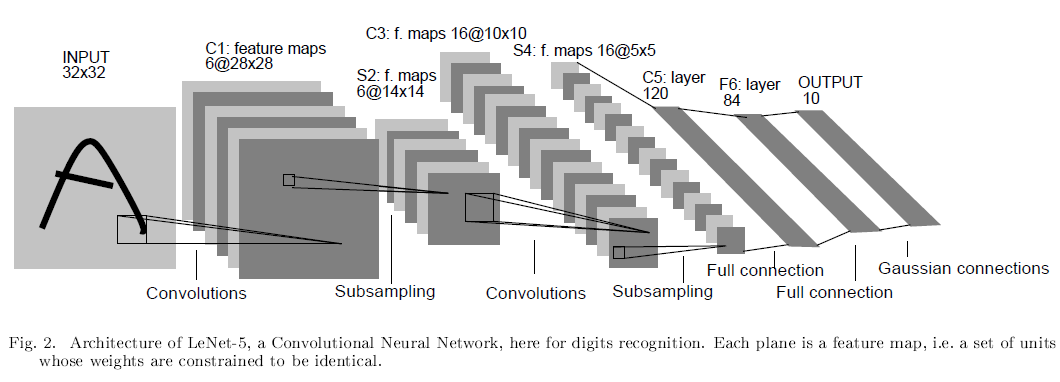
\includegraphics[height=3.5cm]{LeNet-5.png}}
	\end{itemize}
\end{frame}
% ----------------------------------------------------------------------------
\begin{frame}
\frametitle{LeNet-5}
	\small
	\begin{itemize}
		\item domain: hand-writing number recognition
		\item structure:
		\\\hspace{0.5cm}input: 32*32
		\\\hspace{0.5cm}C1: by 6 Conv 5*5, 6*28*28
		\\\hspace{0.5cm}S2: by Weighted Mean Pool 2*2, 6*14*14
		\\\hspace{0.5cm}C3: by 6 Conv 5*5, 16*10*10
		\\(0,1,2)->0
		(1,2,3)->1
		(2,3,4)->2
		(3,4,5)->3
		(4,5,0)->4
		(5,0,1)->5
		(0,1,2,3)->6
		(1,2,3,4)->7
		(2,3,4,5)->8
		(3,4,5,0)->9
		(4,5,0,1)->10
		(5,0,1,2)->11
		(0,1,3,4)->12
		(1,2,4,5)->13
		(0,2,3,5)->14
		(0,1,2,3,4,5)->15
		\\\hspace{0.5cm}S4: by Weighted Mean Pool 2*2, 16*5*5
		\\\hspace{0.5cm}C5: by 16 Conv 5*5, 120*1*1
		\\\hspace{0.5cm}F6: by full connected, 84*1*1
		\\\hspace{0.5cm}Output: by full connected, 10*1*1
	\end{itemize}
\end{frame}
% ----------------------------------------------------------------------------
\begin{frame}
\frametitle{AlexNet}
	\small
	\begin{itemize}
		\item Architecture
			\centerline{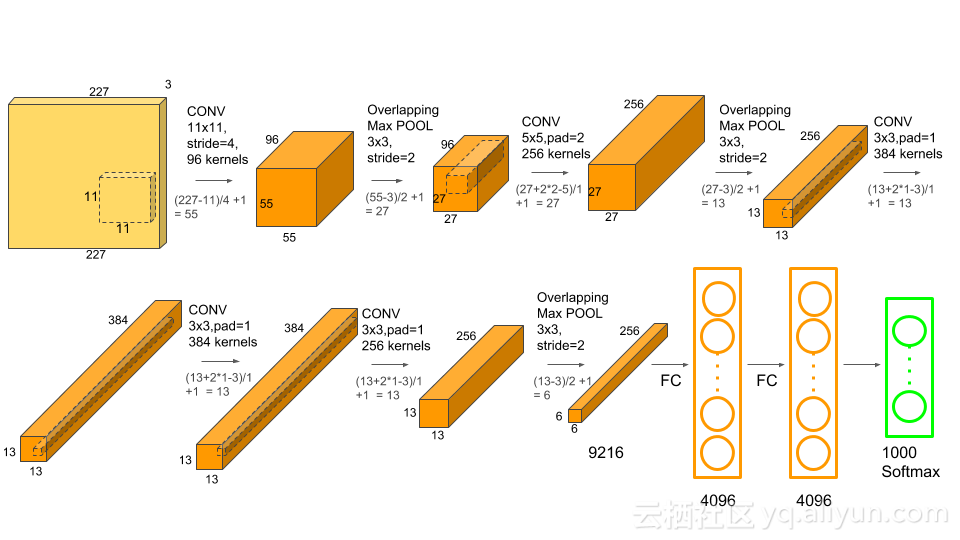
\includegraphics[height=3.5cm]{AlexNet.png}}
			%\centerline{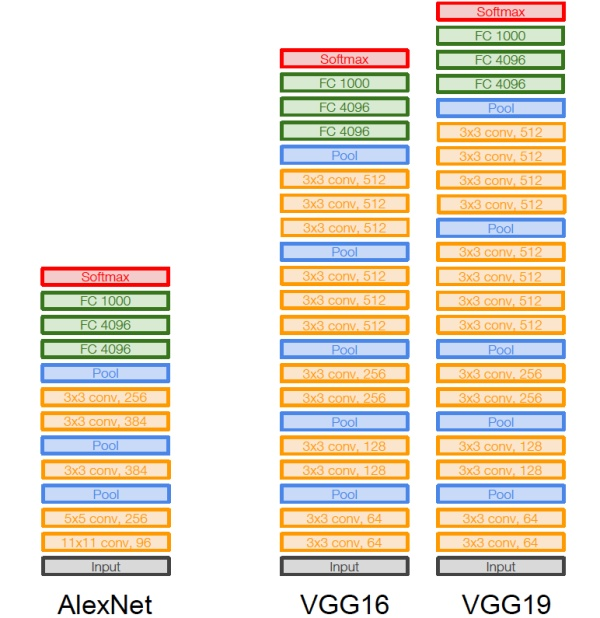
\includegraphics[height=3.5cm]{AlexNet-detail.jpg}}
	\end{itemize}
\end{frame}
% ----------------------------------------------------------------------------
\begin{frame}
\frametitle{VGG}
	\small
	\begin{itemize}
		\item Architecture
			\centerline{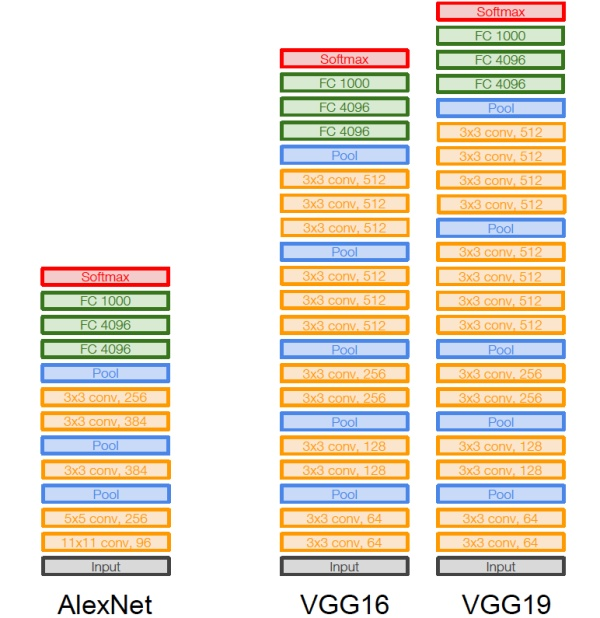
\includegraphics[height=7cm]{AlexNet-detail.jpg}}
	\end{itemize}
\end{frame}
% ----------------------------------------------------------------------------
\begin{frame}
\frametitle{GoogLeNet}
	\small
	\begin{itemize}
		\item Architecture
			\centerline{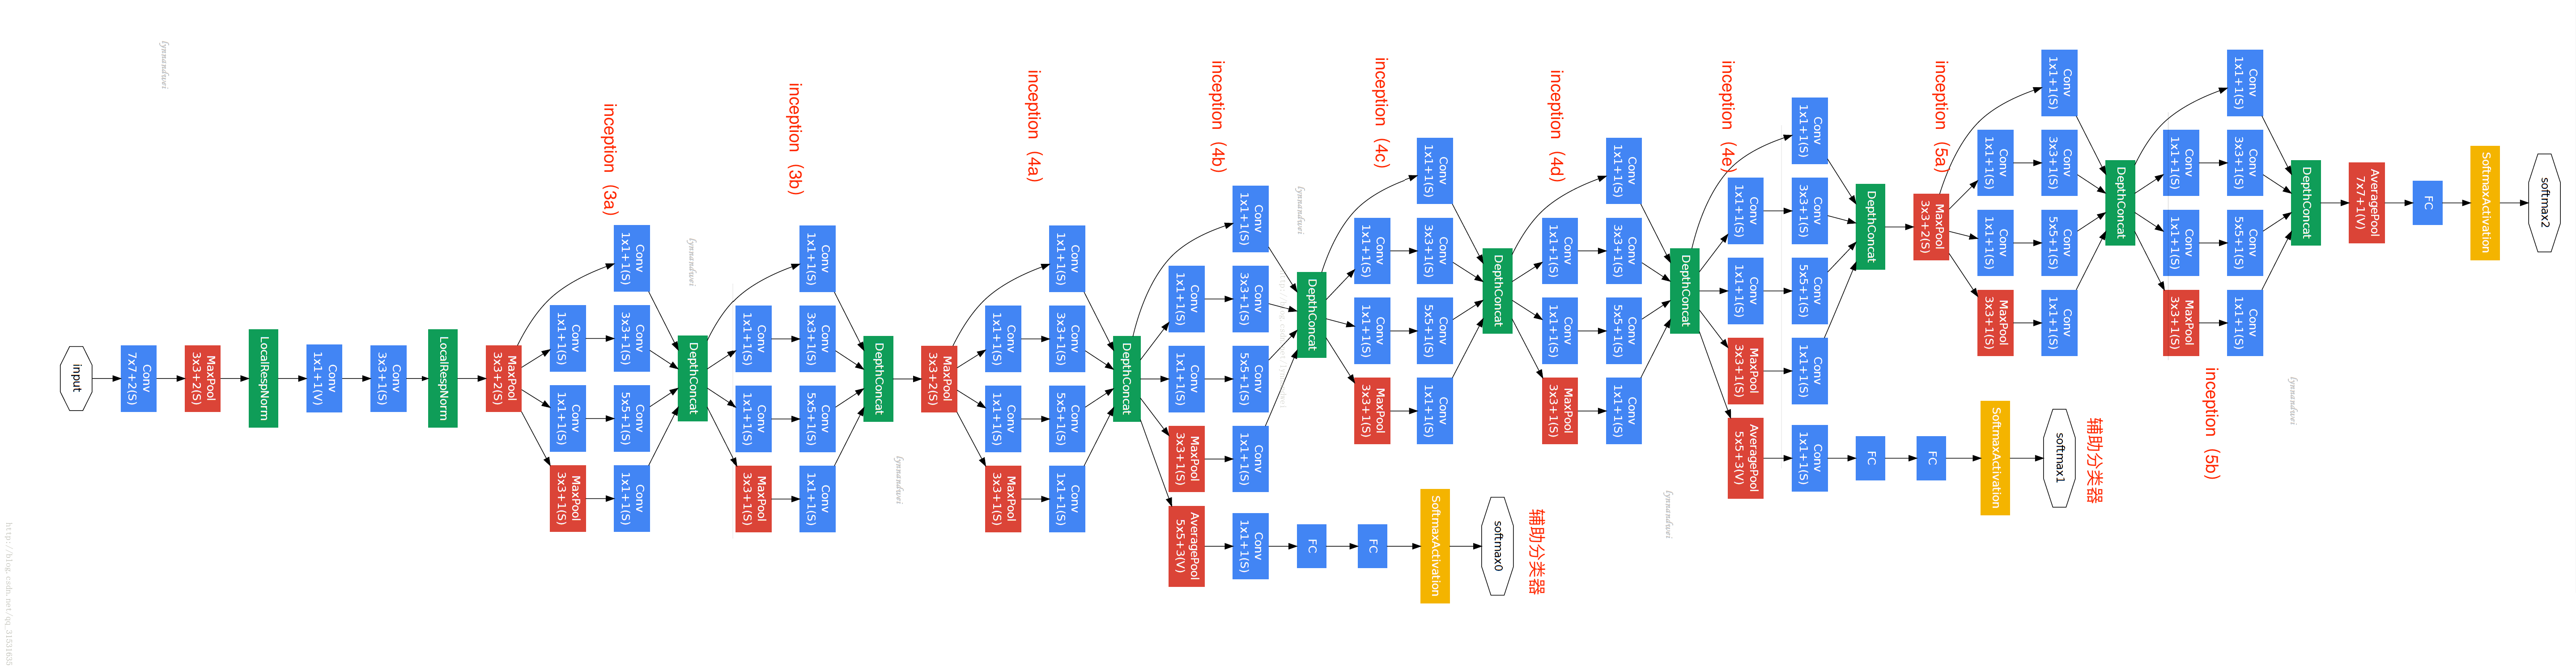
\includegraphics[height=6cm]{GoogLeNet.png}}
	\end{itemize}
\end{frame}
% ----------------------------------------------------------------------------
\begin{frame}
\frametitle{ResNet}
	\small
	\begin{itemize}
		\item Architecture
			\centerline{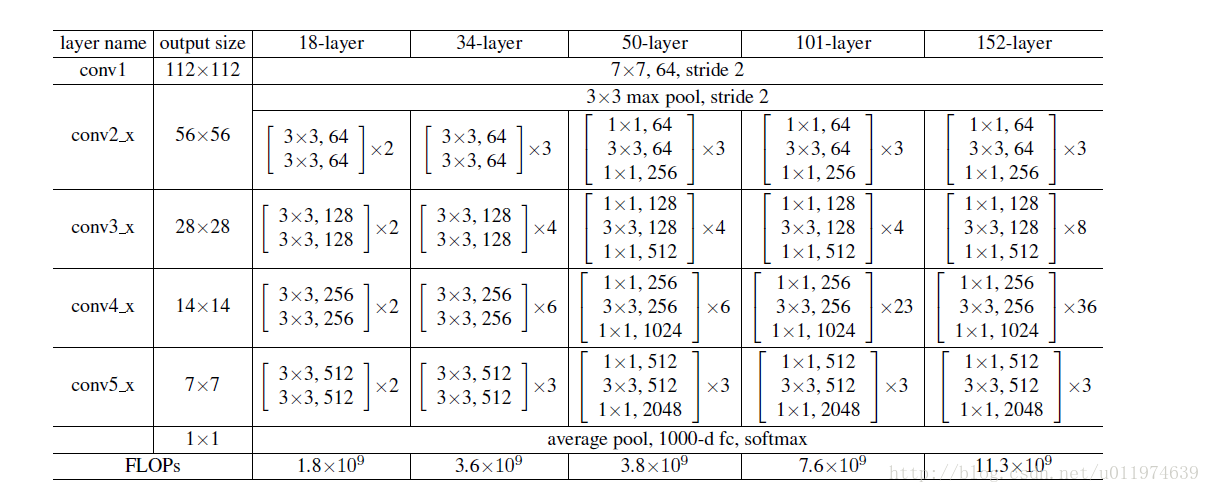
\includegraphics[height=5cm]{ResNet.png}}
	\end{itemize}
\end{frame}
% ----------------------------------------------------------------------------
\ifx\allfiles\undefined
\end{document}
\fi

\ifx\allfiles\undefined
\documentclass[11 pt,t]{beamer}
\geometry{showframe,paperwidth=160mm,paperheight=120mm,margin=5mm,nohead,nofoot,nomarginpar}
%\usetheme[
%bullet=circle,		% Other option: square
%bigpagenumber,		% circled page number on lower right
%topline=true,		% colored bar at the top of the frame 
%]{Zurich}

\usetheme{metropolis}

\usepackage{amsmath}
\usepackage{fontspec,xunicode,xltxtra}
\usepackage{pgf}
\usepackage{tikz}
\usetikzlibrary{patterns}
\usetikzlibrary{plotmarks}
\usetikzlibrary{arrows,decorations.pathmorphing,backgrounds,fit,positioning,shapes,chains}
\definecolor{yellow1}{rgb}{1,0.8,0.2}  
\usepackage{pgfplots}
\pgfplotsset{compat=newest}
\tikzset{elegant/.style={smooth,thick,samples=50,cyan}}
\tikzset{eaxis/.style={->,>=stealth}}

\let\oldequation=\equation
\let\oldendequation=\endequation
\renewenvironment{equation}{\oldequation\textstyle}{\oldendequation}
\setlength{\baselineskip}{0pt}
\renewcommand{\baselinestretch}{0pt}
\setlength{\partopsep}{0pt}
\setlength{\parsep}{0pt}
\setlength{\itemsep}{0cm}
\setlength{\topsep}{0cm}
\setlength{\parskip}{0pt}
\setlength{\lineskip}{0pt}
%\setitemize[1]{itemsep=0pt,partopsep=0pt,parsep=\parskip,topsep=0pt}
%%\usepackage[compatibility=false]{caption}
%%\captionsetup{font={scriptsize}}
\setbeamerfont{caption}{size=\tiny}
\setlength{\abovecaptionskip}{0pt}
\setlength{\belowcaptionskip}{0pt}
\setlength{\abovedisplayshortskip}{0pt}
\setlength{\belowdisplayshortskip}{0pt}
\setlength{\abovedisplayskip}{0pt}
\setlength{\belowdisplayskip}{0pt}
\setlength{\jot}{0pt}
\usepackage{setspace} 
\linespread{1.4}
\fi

\ifx\allfiles\undefined
\begin{document}
\fi
\section{Deep Learning Tricks}
% ----------------------------------------------------------------------------
\begin{frame}
\frametitle{Deep Learning Tricks}
	\small
	\begin{itemize}
		\item Derivative Checking
		\item Gradient Vanishing and Explosion
		\item Data Preparation
			\\\hspace{1cm} Mean-Subtraction and Normalization
			\\\hspace{1cm} PCA and Whitening 
			\\\hspace{1cm} Batch Normalization
		\item Weight Initialization
			\\\hspace{1cm}Pitfall: All Zero Initialization
			\\\hspace{1cm}Small Random Numbers
			\\\hspace{1cm}Calibrating the variances with 1/sqrt(n)
			\\\hspace{1cm}Sparse initialization
			\\\hspace{1cm}Xavier Initialization
		\item Dropout
	\end{itemize}
\end{frame}
% ----------------------------------------------------------------------------
\begin{frame}
\frametitle{Derivative Checking}
	\small
	\begin{itemize}
		\item Check analytical derivative by numerical version. \\
		$f^{\prime} (x)\approx \frac{f(x+h)-f(x-h)}{2h}$
		\item why not $\frac{f(x+h)-f(x)}{h}$ but $\frac{f(x+h)-f(x-h)}{2h}$?
		\\by Tylor expansion at $x$
		\\$\frac{f(x+h)-f(x)}{h}=\frac{1}{h}(f^{(0)}(x)+f^{(1)}(x)h+\frac{1}{2!}f^{(2)}(x)h^2
				+\sum_{n=3}^{\infty}\frac{1}{n!}f^{(n)}h^n-f(x))$
			\\\hspace{1.8cm}$=\frac{1}{h}(f^{(1)}(x)h+\sum_{n=2}^{\infty}\frac{1}{n!}f^{(n)}h^n)$
			\\\hspace{1.8cm}$=f^{(1)}(x)+\frac{1}{h}\sum_{n=2}^{\infty}\frac{1}{n!}f^{(n)}h^n)$
		\\$\frac{f(x+h)-f(x-h)}{2h}=\frac{1}{2h}(f^{(0)}(x)+f^{(1)}(x)h+\sum_{n=2}^{\infty}\frac{1}{n!}f^{(n)}h^n$ 
			\\\hspace{2cm}$-(f^{(0)}(x)+f^{(1)}(x)(-h)+\sum_{n=2}^{\infty}\frac{1}{n!}f^{(n)}(-h)^n))$
			\\\hspace{2cm}$=\frac{1}{2h}(f^{(1)}(x)2h+\sum_{n=2}^{\infty}\frac{2}{(2n-1)!}f^{(2n-1)}2h^{2n-1})))$
			\\\hspace{2cm}$=f^{(1)}(x)+\frac{1}{2h}\sum_{n=2}^{\infty}\frac{2}{(2n-1)!}f^{(2n-1)}2h^{2n-1})))$
			\\$(\frac{f(x+h)-f(x-h)}{2h}-f^{(1)}(x))\thicksim O(h^{2n-1}) \ll  (\frac{f(x+h)-f(x)}{h}-f^{(1)}(x))\thicksim O(h^n)$
	\end{itemize}
\end{frame}
% ----------------------------------------------------------------------------
\begin{frame}
\frametitle{Xavier Initialization}
	\small
	\begin{itemize}
		\item  In order to avoid neurons becoming too correlated and ending up in poor local minimina, it
is often helpful to randomly initialize parameters.One of the most frequent initializations used is called
Xavier initialization.
		\item Given a matrix $A$ of dimension $m * n$, select values $A_{ij}$ uniformly from $[−\epsilon,\epsilon]$, where
		\\\hspace{5cm}$\epsilon = \frac{\sqrt{6}}{\sqrt{m+n}}$
	\end{itemize}
\end{frame}
% ----------------------------------------------------------------------------
\ifx\allfiles\undefined
\end{document}
\fi

%\input{GAN}
\ifx\allfiles\undefined
\documentclass[11 pt,t]{beamer}
\geometry{showframe,paperwidth=160mm,paperheight=120mm,margin=5mm,nohead,nofoot,nomarginpar}
%\usetheme[
%bullet=circle,		% Other option: square
%bigpagenumber,		% circled page number on lower right
%topline=true,		% colored bar at the top of the frame 
%]{Zurich}

\usetheme{metropolis}

\usepackage{amsmath}
\usepackage{fontspec,xunicode,xltxtra}
\usepackage{pgf}
\usepackage{tikz}
\usetikzlibrary{patterns}
\usetikzlibrary{plotmarks}
\usetikzlibrary{arrows,decorations.pathmorphing,backgrounds,fit,positioning,shapes,chains}
\definecolor{yellow1}{rgb}{1,0.8,0.2}  
\usepackage{pgfplots}
\pgfplotsset{compat=newest}
\tikzset{elegant/.style={smooth,thick,samples=50,cyan}}
\tikzset{eaxis/.style={->,>=stealth}}

\let\oldequation=\equation
\let\oldendequation=\endequation
\renewenvironment{equation}{\oldequation\textstyle}{\oldendequation}
\setlength{\baselineskip}{0pt}
\renewcommand{\baselinestretch}{0pt}
\setlength{\partopsep}{0pt}
\setlength{\parsep}{0pt}
\setlength{\itemsep}{0cm}
\setlength{\topsep}{0cm}
\setlength{\parskip}{0pt}
\setlength{\lineskip}{0pt}
%\setitemize[1]{itemsep=0pt,partopsep=0pt,parsep=\parskip,topsep=0pt}
%%\usepackage[compatibility=false]{caption}
%%\captionsetup{font={scriptsize}}
\setbeamerfont{caption}{size=\tiny}
\setlength{\abovecaptionskip}{0pt}
\setlength{\belowcaptionskip}{0pt}
\setlength{\abovedisplayshortskip}{0pt}
\setlength{\belowdisplayshortskip}{0pt}
\setlength{\abovedisplayskip}{0pt}
\setlength{\belowdisplayskip}{0pt}
\setlength{\jot}{0pt}
\usepackage{setspace} 
\linespread{1.4}
\fi

%-----------------------------------------------------------------------------

\ifx\allfiles\undefined
\begin{document}
\fi
\section{Maximum Entropy}
%-----------------------------------------------------------------------------
\begin{frame}
	\frametitle  \ 
	\framesubtitle \   
	\begin{itemize}
		\item Maximum Likelihood solution
		\begin{tiny}
			\begin{table}[!hbp]
				\caption{features and labels($x_2$ is set to be trivial)}
				\begin{tabular}{|c|c|c|}
				\hline
				$y$ & $x_1$ & $x_2$ \\
				\hline
				no	&	sunny	&	hot \\
				no	&	sunny	&	hot \\
				yes	&	overcast&	hot \\
				yes	&	rainy	&	hot \\
				yes	&	rainy	&	hot \\
				no	&	rainy	&	hot \\
				yes	&	overcast&	hot \\
				no	&	sunny	&	hot \\
				yes	&	sunny	&	hot \\
				yes	&	rainy	&	hot	\\
				yes	&	sunny	&	hot	\\
				yes	&	overcast&	hot	\\
				yes	&	overcast&	hot	\\
				no	&	rainy	&	hot	\\
				\hline
				\end{tabular}
			\end{table} 
			\begin{table}[!hbp]
				\caption{probability by maximum likelihood:$y$/$x_1$}
				\begin{tabular}{|c|c|c|c|}
				\hline
					&	sunny	&	rainy	&	overcast \\
				yes	&	40\%	&	60\%	&	100\%	 \\
				no	&	60\%	&	40\%	&	  0\%	 \\
				\hline
				\end{tabular}
			\end{table} 
		\end{tiny}
		\item if $x_2$ is not set to trivial, Maximum Entropy is introduced as follows.
	\end{itemize}
\end{frame}
%-----------------------------------------------------------------------------
%-----------------------------------------------------------------------------
\begin{frame}
\frametitle{Entropy and Conditional Entropy}
\framesubtitle{basic knowledge for the original of  Maximum Entropy method}
	\small	
	\begin{itemize}
		\item In information theory, Entropy is defined to measure unpredictability of random variable $X$.
		\begin{equation}
			H(X)=-\sum_{i=1}^{n}p(x_i)\log_2p(x_i)
		\end{equation}
		\item Conditional Entropy is defined as random variable of $Y$ determined by another random variable of $X$.
		\begin{scriptsize}
		\begin{equation}
			\begin{aligned}{\label{H(y)}}
			H(Y|X)&=\sum_{i=1}^{n}p(x_i)H(Y|X=x_i)\\
				  &=-\sum_{i=1}^{n}p(x_i)\sum_{j=1}^{m}p(y_j|x_i)\log p(y_j|x_i)\\
				  &=-\sum_{i=1}^{n}\sum_{j=1}^{m}p(x_i)p(y_j|x_i)\log p(y_j|x_i)\\
				  &=-\sum_{x,y}p(x)p(y|x)\log p(y|x)
%				  &=-\sum_{i=1}^{n}\sum_{j=1}^{m}p(x_i,y_j)\log p(y_j|x_i)
			\end{aligned}
		\end{equation}
		\end{scriptsize}
	\end{itemize}
\end{frame}
%-----------------------------------------------------------------------------
%-----------------------------------------------------------------------------
\begin{frame}
\frametitle{Optimization Objective}
\framesubtitle{normal step1: build optimization objective}
	\begin{scriptsize}
	\begin{itemize}
		\item input:label vector $Y=(y_1,y_2)$ and feature vector $X=(x_1,x_2)$
		\item output:find $p(y_1|x_1,x_2)$ and $p(y_2|x_1,x_2)$ on the objective of
		\begin{equation}\label{maximumentropy}
			max(H(p(Y|X)))=max(-\sum_{x,y}\widetilde{p}(x)p(y|x)\log p(y|x))
		\end{equation}
		\begin{equation}
			p(y|x)\widetilde{p}({x})f_i(x,y)=\widetilde{p}(x,y)f_i(x,y)\text{, for } i=1,...,k
		\end{equation}
		\begin{equation}{\label{sum(p)}}
			\sum_{y}p(y|x)=1
		\end{equation}
		\item in (6),$\widetilde{p}({x})$ is observed probability of $x$,$\widetilde{p}(x)p(y|x)$ is $p(y|x)$ model's probability of $(x,y)$. (6) means let entropy of model to be maximum.
		\item in (7),$\widetilde{p}(x,y)$ is observed probability of $(x,y)$ in labeled corpus. (7) means let model's probability of $(x,y)$ to be the same to observed.
		\item in (7),$f_i(x,y)$ is feature function, i.e. how much does $y$ is affected by $x$. If $x$ and $y$ appears at the same time $f_i(x,y)=1$, else $f_i(x,y)=0$. 
		\item in (8),$\sum_{y}p(y|x)$ means if the same $x$ will effected different $y$, the summary of probability of $y$ must be 1. 
	\end{itemize}
	\end{scriptsize}
\end{frame}
% ----------------------------------------------------------------------------
\section{Lagrange Dual Problem}
% ----------------------------------------------------------------------------
\begin{frame}
\frametitle{Lagrange Dual Problem Optimization}
\framesubtitle{use mathematical tool to convert constrainted to unconstrainted optimization}
	\begin{scriptsize}
		\begin{itemize}
			\item Lagrange function associated with Maximum Entropy objective function is defined as
			\begin{equation}\label{L(p)}
				L(p(y|x),\lambda_i,\lambda_0)=H(p)+\sum_{i=1}^{k}(\lambda_if_i(x,y)(p(y|x)\widetilde{p}({x})-\widetilde{p}(x,y)))+\lambda_0(\sum_{y}p(y|x)-1)
			\end{equation}
			\item The stationary point of Lagrange function is the same to original Maximum Entropy objective function.
			\begin{equation}
				\frac{\partial{L}}{\partial{\lambda_i}}=0 \Rightarrow 
				p(y|x)\widetilde{p}({x})f_i(x,y)=\widetilde{p}(x,y)f_i(x,y)\text{, for } i=1,...,k
			\end{equation}  
			\begin{equation}
				\frac{\partial{L}}{\partial{\lambda_0}}=0 \Rightarrow
				\sum_{y}p(y|x)=1
			\end{equation}
			\begin{equation}\label{p=lambda}
				\frac{\partial{L}}{\partial{p}}=0 \Rightarrow \frac{\partial{H(p)}}{\partial{p}}=0
			\end{equation}
			\item from \ref{H(y)} ($H(Y|X)=-\sum_{x,y}\widetilde{p}(x)p(y|x)\log p(y|x)$), \ref{L(p)}, \ref{p=lambda}, we can have
			\begin{equation}
				\frac{\partial{L}}{\partial{p}}=-\widetilde{p}(x)(\log p(y|x) + 1)+\sum_{i=1}^{k}(\lambda_if_i(x,y)\widetilde{p}({x})+\lambda_0=0
			\end{equation}
			\begin{equation}
				p^*(y|x)=e^{\sum_{i=1}^{k}\lambda_if_i(x,y)-\frac{\lambda_0}{\widetilde{p}(x)}-1}
			\end{equation}
		\end{itemize}
	\end{scriptsize}
\end{frame}
% ----------------------------------------------------------------------------
\begin{frame}
	\begin{scriptsize}
		\begin{itemize}
			\item by \ref{sum(p)}, we can remove $\lambda_0$, in the following way 
				\begin{equation}
					e^{\frac{\lambda_0}{\widetilde{p}(x)}+1}=\sum_{y}e^{\sum_{i=1}^{k}\lambda_if_i(x,y)}
				\end{equation}
				\begin{equation}\label{p}
					\left\{
						\begin{aligned}
					 	&p^*(y|x)=\frac{e^{\sum_{i=1}^{k}\lambda_if_i(x,y)}}{Z(x)}\\
						&Z(x)=\sum_{y}e^{\sum_{i=1}^{k}\lambda_if_i(x,y)}
						\end{aligned}
					\right.
				\end{equation}
				\item by \ref{p}, we have simplified $L(p(y|x),\lambda_i,\lambda_0)$ to
				\begin{equation}\label{duality}
					L(\lambda)=\sum_{x,y}\widetilde(p)(x)p^*(y|x)\log Z(x)-\sum_{i=1}^k\widetilde{p}(x,y)\sum_{x,y}\lambda_if_i(x,y)
				\end{equation}
				\item \ref{duality} is a complex function of $\lambda$, by finding the stationary point of this function we can find the possible maximum point of \ref{maximumentropy}. We can define primal problem is:
				\begin{equation}\label{primal}
					\left\{
						\begin{aligned}
							&H(p(Y|X))=-\sum_{x,y}\widetilde{p}(x)p(y|x)\log p(y|x)\\
							&\frac{\partial{H(p)}}{\partial{p}}=0
						\end{aligned}
					\right.
				\end{equation}
		\end{itemize}
	\end{scriptsize}
\end{frame}
% ----------------------------------------------------------------------------
\begin{frame}
	\frametitle{Lagrange Dual Problem}
	\framesubtitle{to understand the property of Lagrange dual function}
	\begin{scriptsize}
	\begin{itemize}	
		\item General Lagrange dual problem of \ref{primal} is as follows
		\begin{equation}
			\left\{
				\begin{aligned}
					&\frac{\partial{L}}{\partial{\lambda}}=0\\
					&L(\lambda)=\sum_{x,y}\widetilde{p}(x)p^*(y|x)\log Z(x)-\sum_{i=1}^k\widetilde{p}(x,y)\sum_{x,y}\lambda_if_i(x,y)\\
					&p^*(y|x)=\frac{1}{Z_\lambda(x)}e^{\sum_i\lambda_if_i(x,y)}\\
					&Z_\lambda(x)=\sum_ye^{\sum_i\lambda_if_i(x,y)}
				\end{aligned}
			\right.
		\end{equation}
		\item In our case, $\widetilde{p}(x)=1$, and $\widetilde{p}(x,y_1)=0.4$, and $\widetilde{p}(x,y_2)=0.6$, and $\lambda_1$ is for $f(y_1|x)$, and $\lambda_2$ is for $f(y_2|x)$
		\begin{equation}\label{sample}
			\left\{
				\begin{aligned}
					&Z_\lambda(x)=e^{\lambda_1}+e^{\lambda_2}\\
					&p^*(y_{1 or 2}|x)=\frac{e^{\lambda_{1 or 2}}}{e^{\lambda_1}+e^{\lambda_2}}\\
					&L(\lambda)=-\log(e^{\lambda_1}+e^{\lambda_2})+(0.4\lambda_1+0.6\lambda_2)\\
					&H(p(Y|X))=-(\frac{\lambda_{1}e^{\lambda_{1}}+\lambda_{2}e^{\lambda_{2}}}{e^{\lambda_1}+e^{\lambda_2}}-\log(e^{\lambda_1}+e^{\lambda_2}))\\
					%&\sum_{i=1}^{k}(\lambda_if_i(x,y)(p(y|x)\widetilde{p}({x})-\widetilde{p}(x,y)))=\frac{\lambda_{1}e^{\lambda_{1}}+\lambda_{2}e^{\lambda_{2}}}{e^{\lambda_1}+e^{\lambda_2}}-0.4\lambda_1-0.6\lambda_2
				\end{aligned}
			\right.
		\end{equation}
	\end{itemize}
	\end{scriptsize}
\end{frame}

% ----------------------------------------------------------------------------
%\begin{frame}
%\centering 
%	\begin{tikzpicture}
%		\begin{axis}[xstep=0.1,ystep=0.1]
%		\addplot3[surf,domain=0.001:1]
%			{-ln(exp(x)+exp(y))+0.4*x+0.6*y};
%		\end{axis}
%	\end{tikzpicture}
%	$\lambda(x,y)=-\log(e^x+e^y)+0.4x+0.6y$
%\end{frame}
%\begin{frame}
%	\centering
%	\begin{tikzpicture}
%		\begin{axis}[xstep=0.1,ystep=0.1]
%		\addplot3[surf,domain=0.001:1]
%			{-((x*exp(x)+y*exp(y))/(exp(x)+exp(y))-ln(exp(x)+exp(y)))};
%		\end{axis}
%	\end{tikzpicture}
%	$H(p)=-(\frac{x*e^x+y*e^y}{e^x+e^y}-\log(e^x+e^y))$
%\end{frame}
% ----------------------------------------------------------------------------
%\begin{frame}
%	\frametitle{Another Understanding of Lagrange Dual Function}
%	\framesubtitle{a graphical understanding of previous sample}
%	\begin{scriptsize}
%	\begin{itemize}	
%		\item $L(\lambda,x_1,x_2)=-(x_1\log(x_1)+x_2\log(x_2))+\lambda_1(x_1-0.4)+\lambda_2(x_2-0.6)$ can be seen as:\\
%		 the maximum distance between surface of $x_1\log(x_1)+x_2\log(x_2)$ and plain of $\lambda_1(x_1-0.4)+\lambda_2(x_2-0.6)$
%	\end{itemize}
%	\end{scriptsize}
%	\centering 
%	\begin{tikzpicture}
%		\begin{axis}[xstep=0.1,ystep=0.1]
%		\addplot3[surf,domain=0.001:1]
%			{x*ln(x)+y*ln(y)};
%
%		\addplot3[green,domain=0:1]
%			{0.223144*(x-0.4)-0.182322*(y-0.6)};
%		\end{axis}
%	\end{tikzpicture}
%\end{frame}
% ----------------------------------------------------------------------------
\begin{frame}
	\frametitle{Conjugate Function}
	\framesubtitle{another understanding of Lagrange dual function}
	\begin{scriptsize}
	\begin{itemize}
		\item From the graphical understanding of previous page, we define conjugate function as
		\begin{equation}
			f^*(y)=\sup_{x\in \text{dom} f(x)}(yx-f(x))
		\end{equation}
		\item from the definition of $f^*(y)$, we can know when $y=f'(x)$, supermum is got 
			\begin{equation}
				f^*(y)=yf'(x)-f(f'(x))
			\end{equation}
   		\item some conjugate of convex functions are as follows
		\begin{equation}\label{conjugate}
			\begin {aligned}
				&f(x)=ax+b \rightarrow f^*(y)=ya-ay+b=b \\
				&f(x)=-\log x \rightarrow f^*(y)=y(-\frac{1}{y})+\log (-\frac{1}{y})=-\log (-y)-1\\
				&f(x)=x\log x \rightarrow f^*(y)=ye^{y-1}-e^{y-1}\log{e^y-1}=e^{y-1}
			\end {aligned}
		\end{equation}
		\item use \ref{conjugate} in \ref{L(p)}, we can get Lagrange dual at once
			\begin{equation}
				L(\lambda)=b\sum_{i=1}^{k}{\lambda_i}-\log(\sum_{i=1}^{k}e^{\lambda_i})
			\end{equation}
		\item it matches the result in \ref{sample} 
	\end{itemize}
	\end{scriptsize}
\end{frame}
% ----------------------------------------------------------------------------
\section{Optimization Algorithm}
% ----------------------------------------------------------------------------
\begin{frame}
	\frametitle{Optimization Algorithm}
	\framesubtitle{find $\lambda$ for dual and primal problem}	
	\begin{scriptsize}
	\begin{itemize}
		\item There are multiple unconstrained optimization algorithm to resolve Lagrange Dual problem $\frac{\partial L(\lambda)}{\partial \lambda}=0$
		\item Gradient Decent Method
		\begin{equation}
			\left\{
			\begin{aligned}
			&\lambda_i^{n+1}=\lambda_i^{n}+C\Delta\lambda_i \\
			&\Delta\lambda_i=\sum_{x,y}\widetilde{p}(x,y)f_i(x,y)-\sum_{x}\widetilde{p}(x)\sum_{y}p^*(y|x)f_i(x,y)
			\end{aligned}
			\right.
		\end{equation}
		\item GIS (Generative Iterative Scaling)
		\begin{equation}
			\lambda_i^{n+1}=\lambda_i^{n}+\frac{1}{C}\log\frac{\sum_{x,y}\widetilde{p}(x,y)f_i(x,y))}{\sum_{x}\widetilde{p}(x)\sum_{y}p^*(y|x)f_i(x,y)}
		\end{equation}
		\item IIS (Improved Iterative Scalling)
		if $\sum_if_i(x,y)$ is constant,$\lambda_i$ is got by \ref{constant}, else by \ref{variable}
		\begin{equation}\label{constant}
			\lambda_i=\frac{1}{\sum_if_i(x,y)}\log\frac{\sum_{x,y}\widetilde{p}(x,y)f_i(x,y)}{\sum_{x}\widetilde{p}(x)\sum_{y}p^*(y|x)f_i(x,y)}
		\end{equation}
		\begin{equation}\label{variable}
			\left\{
			\begin{aligned}
			&\lambda_i^{n+1}=\lambda_i^{n}+\Delta\lambda_i \\
			&\sum_{x,y}\widetilde{p}(x,y)f_i(x,y)-\sum_{x}\widetilde{p}(x)\sum_{y}p^*(y|x)f_i(x,y)e^{\Delta\lambda_i\sum_if_i(x,y)}=0
			\end{aligned}
			\right.
		\end{equation}
		\end{itemize}
	\end{scriptsize}
\end{frame}
% ----------------------------------------------------------------------------
\begin{frame}
\begin{equation} \alpha=arg\;
\underset{\alpha\geq 0}{\min}h(\alpha)=arg\;\underset{\alpha\geq 0}{\min}f(x_k+\alpha d_k) \end{equation}\\

\(h(\alpha)\)
\(h'(\alpha)=\nabla f(x_k+\alpha d_k)^Td_k=0\)。\(d_k\)
\(f(x_k)\)
\(x_k\)
\(h'(0)\leq 0\)
\(\hat{\alpha}\)
\(h'(\hat{\alpha})>0\)
\(\alpha^{\star}\in [0,\hat{\alpha})\)
\(h'(\alpha^{\star})=0\)
\(\alpha^{\star}\)
\end{frame}
% ----------------------------------------------------------------------------
\ifx\allfiles\undefined
\end{document}
\fi

% ----------------------------------------------------------------------------
%\begin{frame}
%\begin{thebibliography}{}
%\tiny
%\bibitem{Maximum Likelihood}Maximum Likelihood, Huang Yuefeng
%\end{thebibliography}
%\end{frame}

% ----------------------------------------------------------------------------
%\usebackgroundtemplate{
%	\includegraphics[width=\paperwidth,
%		height=\paperheight]{aletsch}
%}
\begin{frame}
\
\centering \Large \textcolor{black}{Questions?}

\end{frame}
\usebackgroundtemplate{}
% ----------------------------------------------------------------------------


\end{document}
